% !TEX root = ../Thesis.tex
\chapter{Evaluation}

In this section we talk about the evaluation as a whole. We take a look at the phrase set we used, how we carried it out, the results that can be observed and compare it to existing results.

\section{MacKenzie Phrase Set}
For the evaluation we use the MacKenzie Phrase Set\footnote{http://www.yorku.ca/mack/PhraseSets.zip}. This is a set of 500 phrases. According to MacKenzie and Soukoreff \cite{10.1145/765891.765971}, such a phrase set should use phrases of moderate length that are easy to remember and representative for the target language.\\
The phrases of the MacKenzie Phrase Set do not contain any punctuation. Some of them use uppercase characters, but the authors mention, that participants can also be instructed to ignore the case of the characters.\\
Some statistics for the whole phrase set, also found in the original paper \cite{10.1145/765891.765971}: The MacKenzie phrase set consists of 500 phrases that have a minimum length of 16, a maximum length of 43 and an average length of 28.61 characters. On the whole, 2712 words were used, which consist of 1163 unique words. A phrase consists of a minimum of 1, a maximum of 13 and on average of 4.46 words.

\section{Task of the Participants}
The task of the participants is to copy 15 phrases from the MacKenzie Phrase Set. As they are not in a specific order, e.g. alphabetic order, we decide to take adjacent phrases and not random ones.
\begin{figure}[H]
    \centering
    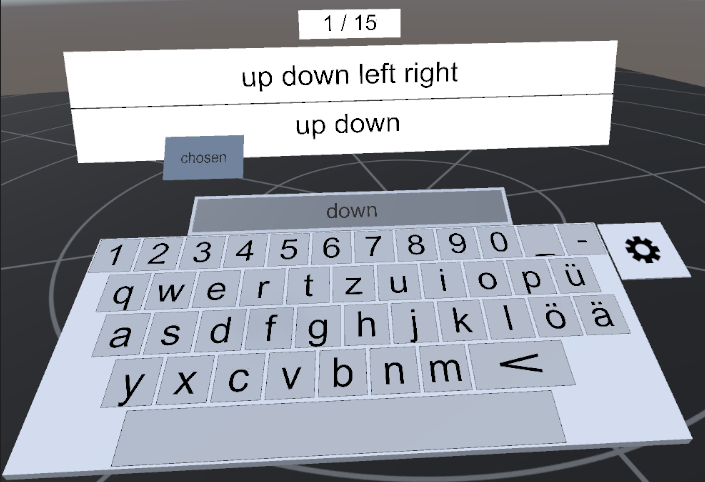
\includegraphics[width=0.5\textwidth]{WGKEvaluationScene.png}
    \caption{The textfield a participant sees. The phrase to copy is on top, the lower textfield displays the words the participant wrote.}
    \label{fig:eval_scene}
\end{figure}
The participants see two text fields as shown in \Cref{fig:eval_scene}. On the top is the phrase to copy, on the bottom the words/phrase they write. If the given phrase matches the phrase the participant wrote, a tone sounds, such that the participants know when they finish one specific phrase. After that, a new phrase appears until 15 phrases are correctly inputted. If an incorrect word is entered, the participant either can use the word suggestions \cref{fig:write_suggestions:write_suggestions2} or delete the wrong word and try to write it again. If a mistake is only noticed later on, the participants have to remove all words and characters up to and including the wrong word by using the backspace button.\label{sec:eva_task} After this first step, in a second step, the participants get introduced to the scaling and the ``add word'' functions, which they could test afterwards. This is important, because we want to know if they find these functions useful and well implemented. The last step of the evaluation is to fill a questionnaire. First, it has some general questions about the participant's experience in VR. Then there is a block of twelve questions. The first ten are from the system usability scale, but the first one is changed a bit. The last two questions are for the previously mentioned functions. Per question, there are five possibilities to choose from, from 1 (strongly disagree) to 5 (strongly agree). The questions are structured in such a way that if the user is highly satisfied with everything, they would alternately make a cross at the 5 and 1.

\section{Carry-out}
To carry out the evaluation, we used two different VR systems. One was a setup with a HTC vive and HTC vive controllers. The other one included an Oculus Rift headset with corresponding controllers. Even though these are two different systems, it did not change much for the participants. In fact, only the controllers and their buttons differ a bit.\\
The participants consist of volunteers including computer science students, friends and family members. In total, eleven people got in touch with us and participated at our evaluation. Every participant got the same explanation to give everybody the same foundation of knowledge.
Participants were provided the following information:\\
If they are close enough to the keyboard, then the color gets a bit brighter, and they are in the keyboard's hitbox. The keyboard is movable if they press and hold the controller's grip button in the hitbox of the keyboard. If they release it, the keyboard gets static again and stays where it got put.\\
To write, they also have to be in the hitbox of the keyboard but not pressing and holding the grip button, but the trigger button. While pressing, they can make a gesture over the characters of the keyboard. They will see a red line where they move. If they release the trigger button, the system tries to find the best matching word and puts it in the text field. If they do a gesture and a word longer than one character is written, a space is automatically put behind the word. Single characters can be written by clicking on the key of the intended character. If they write a single character, no space is put behind it, and they have to do it on their own. In the English language, this is particularly important for the words ``I'' and ``a''. If they make a gesture and a word is written, there may be one to four other choosable words displayed in buttons. They can pick from them if the word written in the text field is not the intended one. The participants were warned about the word ``the'', because all the time ``thee'' would be written, therefore they would have to correct it every time.\\
If they use the backspace button after writing a word, the whole word gets deleted and afterwards only single characters get deleted.\\
They have enough time, and they should not hurry, but rather make sure that the inputted words are correct. Because if they are not correct, they have to use the backspace a lot of times, and they lose a lot of time.

In total for the eleven participants, 165 phrases were used. The average word length is 4.16 with the minimum length of 1 and a maximum length of 12 characters. In total, these phrases contain 856 words, 460 of which are unique. Before the carry-out we made sure that all the words in these phrases were in our word lexicon, such that the participants could write every word with a gesture.
\section{Results}
Now, we talk about the results and some statistics we gained through the evaluation and compare them to exisiting results.\\

\subsection{System Usability Scale}
First, we begin with the results of the SUS questions. Note that we slightly changed the first question by appending ``when I work in VR''. These ten questions were:\\
1. I think that I would like to use this system frequently when I work in VR\\
2. I found the system unnecessarily complex\\
3. I thought the system was easy to use \\
4. I think that I need the support of a technical person to be able to use this system\\
5. I found the various functions in this system were well integrated\\
6. I thought there was too much inconsistency in this system\\
7. I would imagine that most people would learn to use this system very quickly\\
8. I found the system very cumbersome to use\\
9. I felt very confident using the system\\
10. I needed to learn a lot of things before I could get going with this system
\iffalse
\begin{table}[ht!]
    \centering
    \caption{Results from the System Usability Scale (SUS) from the questionnaire (first ten questions)}
    \begin{tabular}{cccc} \toprule
        question&average score&perfect possible score&$\sigma$\\ \midrule
        1 & 4.27 & 5.0 & 0.445\\ 
        2 & 1.09 & 1.0 & 0.287\\
        3 & 4.64 & 5.0 & 0.481\\ 
        4 & 1.27 & 1.0 & 0.617\\
        5 & 4.64 & 5.0 & 0.481\\
        6 & 1.64 & 1.0 & 0.979\\
        7 & 4.64 & 5.0 & 0.481\\
        8 & 1.45 & 1.0 & 0.498\\
        9 & 4.09 & 5.0 & 0.514\\
        10 & 1.55 & 1.0 & 0.656\\
        \bottomrule
    \end{tabular}
    \label{tab:table}
\end{table}
\fi
\begin{figure}[H]
    \noindent
    \makebox[\textwidth][c]{
        \centering
        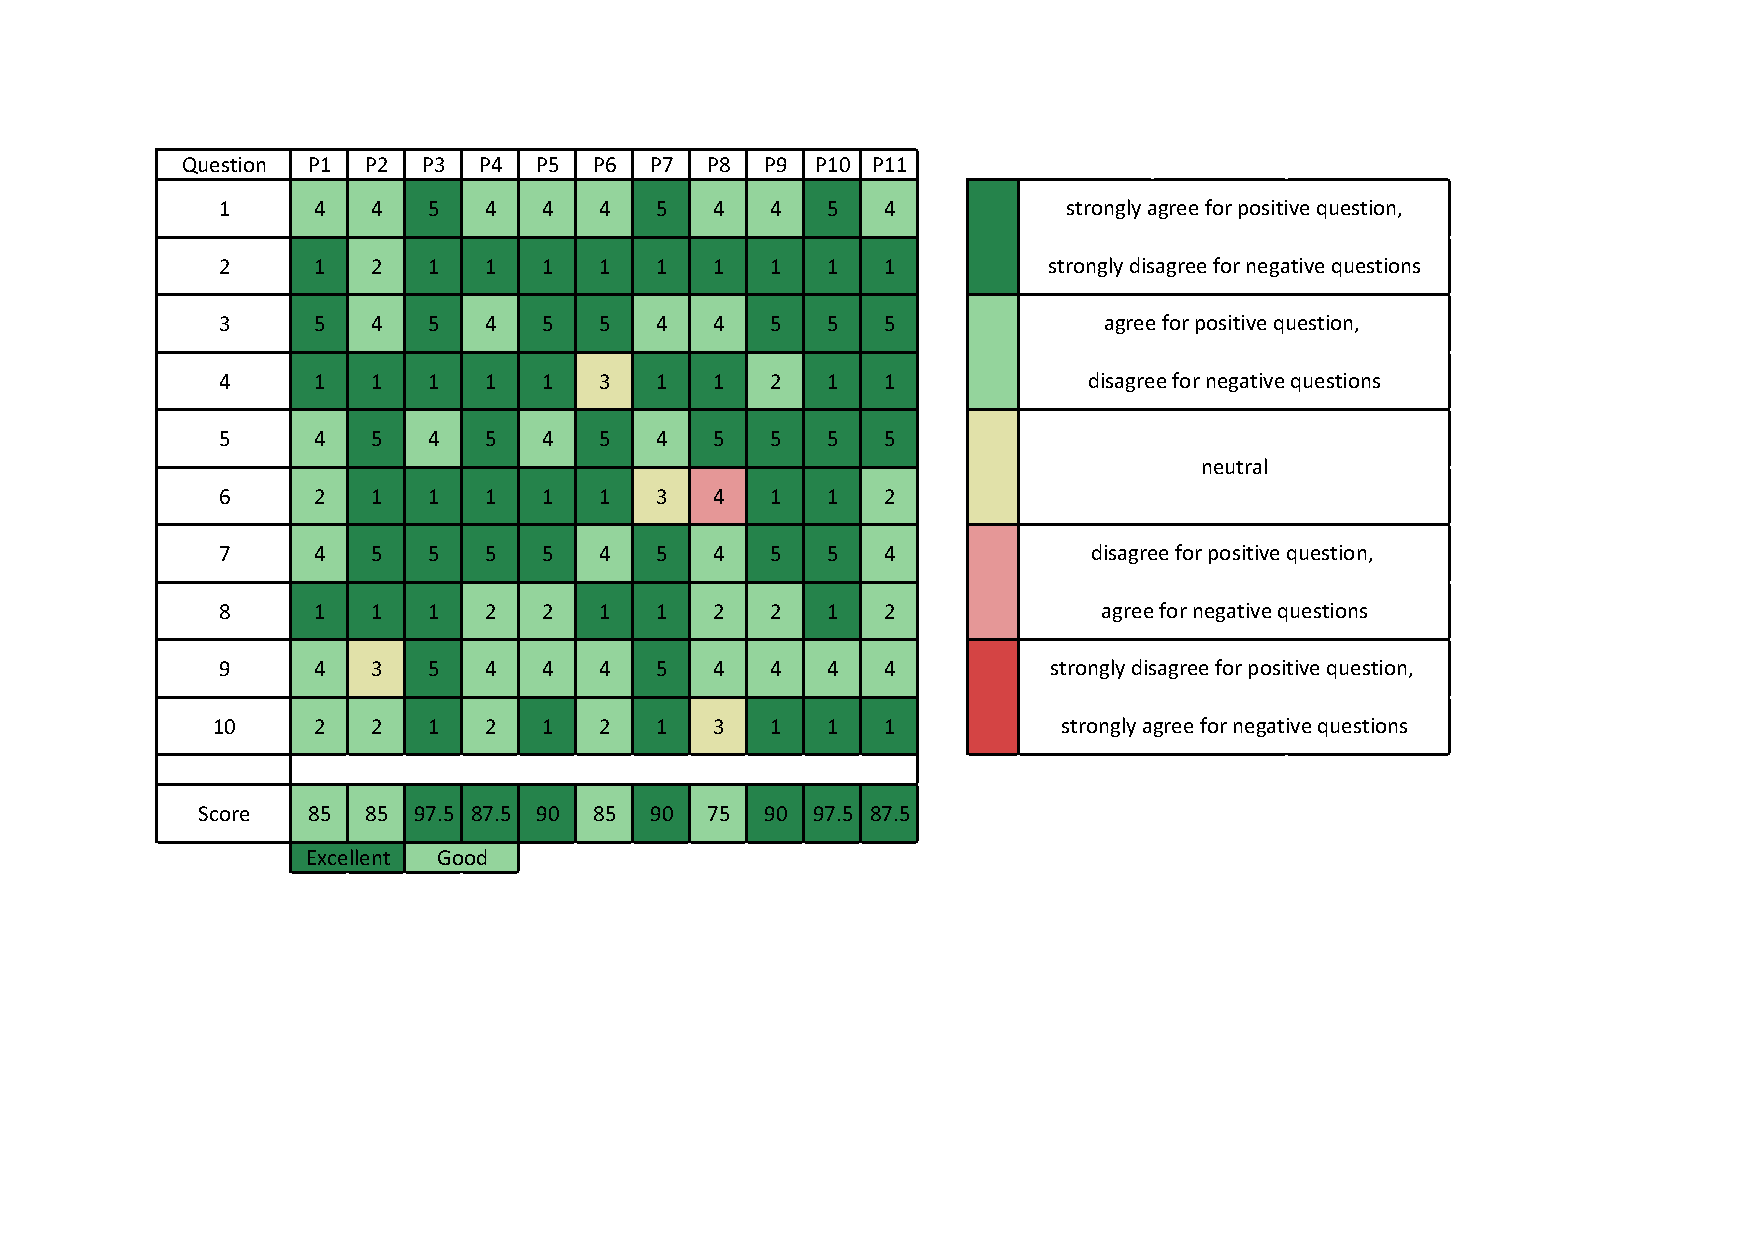
\includegraphics[width=1.3\textwidth]{SUS_scoring.pdf}\hspace{-4em}
    }
    \vspace*{-10em}
    \caption{System Usability Scale with all the given points per question from every participant}
    \label{fig:SUS_score}
\end{figure}

In \Cref{fig:SUS_score} green fields mark positive responses to questions, red ones negative responses and yellow ones neutral feedback. All in all, we can see a lot of green fields, which means the feedback to the SUS questions is quite good. Question 9 got the worst score, but with it being a 4.09 out of 5, it is still fairly good. From the average values for each question, we can calculate a usability score. Every question with an even number is a negative one. This means, the highest possible score for them is 1 or ``strongly disagree''. For the other questions, a score of 5 or ``strongly agree'' is the best possible score. So, from the odd numbered questions 1 has to be subtracted from the average score. For the even numbered questions, the average score needs to be subtracted from 5. At the end, these ten newly calculated values have to be summed up and multiplied by 2.5. Our calculated usability score is 88.18. This is a high score, because from a score of 85.5 points, one talks about an excellent system usability.\\
We also have two additional questions about the scale and the ``add word'' function:\\
11. The function to add words is well implemented and easy to use\\
12. The function to scale the keyboard is unnecessary\\
Question 11 got a score of 4.55 out of 5 and question 12 got a score of 2.18, whereby 1 would be ideal. We conclude from these two questions, that the ``add word'' function makes a good impression whereas the scale function does not perform so well.\\

\subsection{Writing Speed}
One important thing of our evaluation is to find out, how fast users can write with our word-gesture keyboard. As unit to measure these values, we take the ``words per minute'' WPM. We calculate the WPM with following formula: 

\begin{equation}
    WPM = \frac{\mid T \mid}{S} \times 60 \times \frac{1}{5}
\end{equation}
where $T$ is the transcribed text, hence these are the phrases a participant had to write. Therefore, $\mid T \mid$ is the number of characters in the transcribed text. Finally, $S$ is the time in seconds they used to write all 15 phrases.\\

\begin{table}[ht!]
    \centering
    \caption{Average WPM, lowest WPM and highest WPM per participant. For the first three, we failed to record all data.}
    \begin{tabular}{cccc} \toprule
        participant&average WPM&lowest WPM&highest WPM\\ \midrule
        1 & 11.457 & - & -\\ 
        2 & 12.19 & - & -\\
        3 & 13.055 & - & -\\ 
        4 & 11.609 & 5.3 & 25.5\\
        5 & 12.578 & 6.83 & 21.65\\
        6 & 10.285 & 5.27 & 19\\
        7 & 12.423 & 6.1 & 24.41\\
        8 & 16.056 & 8.28 & 30.74\\
        9 & 13.363 & 7.96 & 24.15\\
        10 & 17.118 & 7.98 & 24.45\\
        11 & 10.067 & 4.71 & 14.55\\
        \bottomrule
        average&12.75&6.55&23.06\\
        \bottomrule
    \end{tabular}
    \label{tab:WPM}
\end{table}
In Table \ref{tab:WPM} we can see how fast on average the participants were able to write their 15 phrases. We do also list the lowest and highest value. To understand the values of Table \ref{tab:WPM} a bit better, we make a so-called boxplot for every participant, for whom we have the necessary data.
\begin{figure}[H]
    \centering
    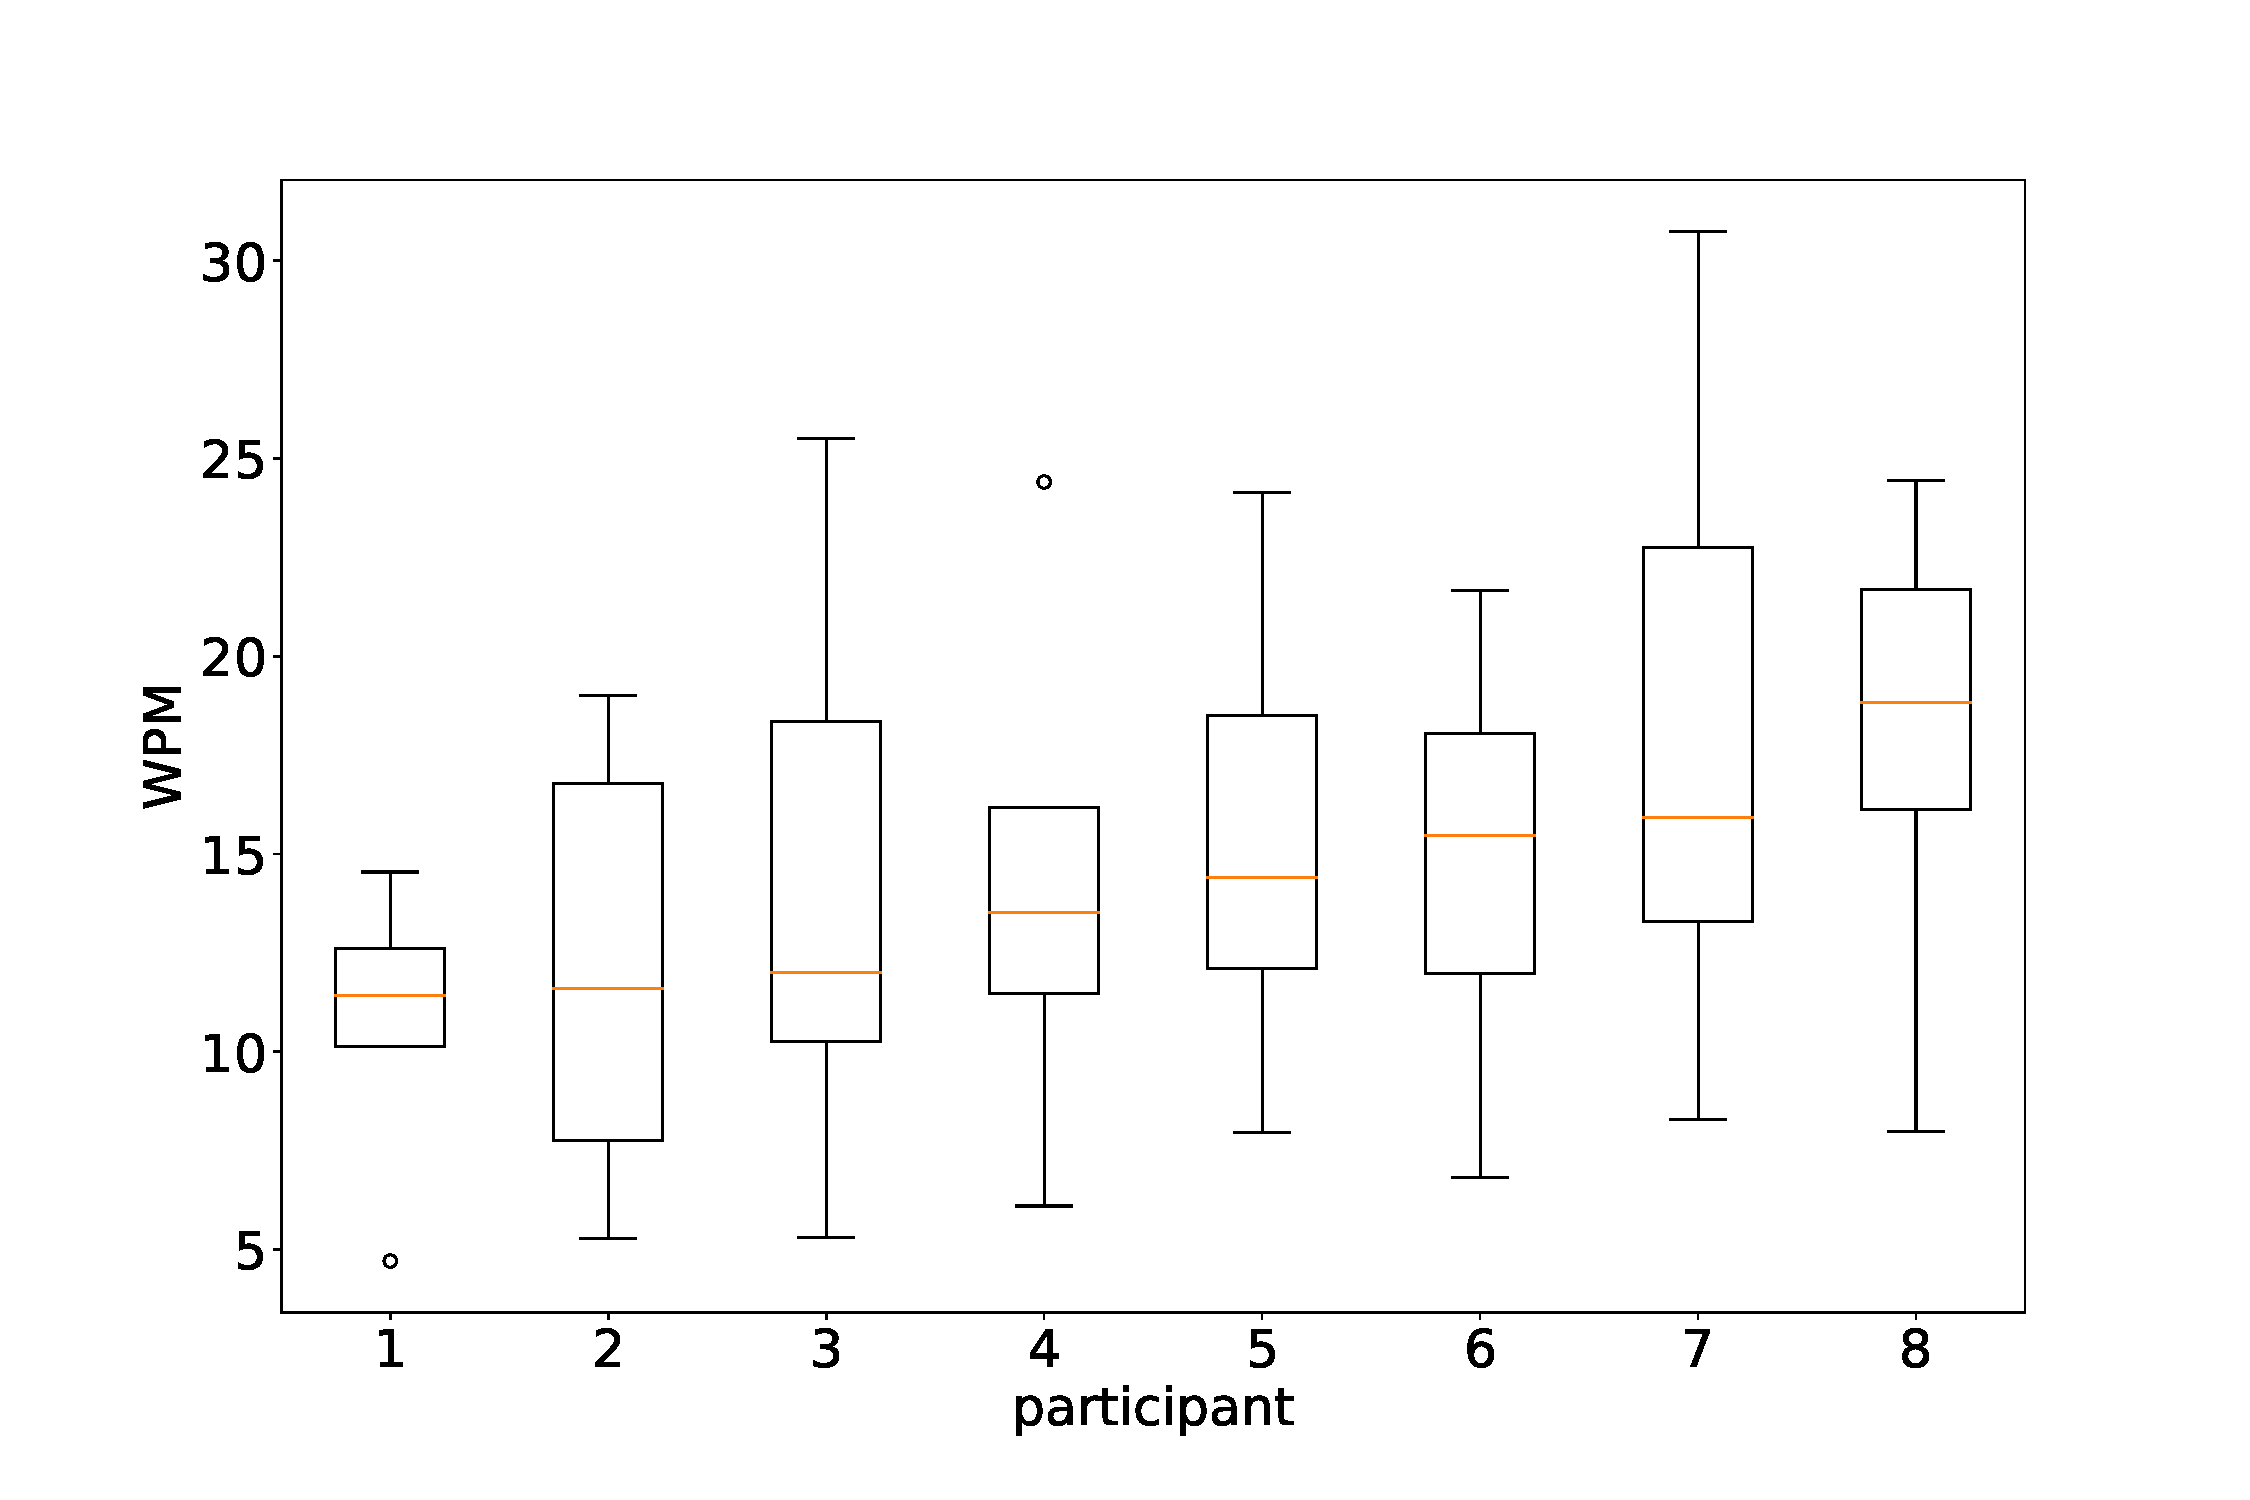
\includegraphics[width=0.9\textwidth]{wpm_boxplot.pdf}
    \caption{for participants 4-11: The upper and lower whiskers (or the outliers if the values are too extreme) show the maximum and minimum, the boxes show the 25\% and 75\% quartiles and the orange lines mark the median values. Each box corresponds to one participant.}
    \label{fig:WPM}
\end{figure}
We can see in fig \ref{fig:WPM}, the higher the participant's median, most of the time, the higher the lowest WPM value. The lowest WPM values mostly come about because a participant made a mistake and had to delete a lot and basically write the phrase two times. On the other hand, most of the highest WPM values come about because a participant made no mistake in writing the phrase. The rectangle in the middle of the two bars shows how consistent or inconsistent a participant's writing speed was. The lower bound is the 25\% quartile, the upper bound the 75\% quartile. This means, if the rectangle is shorter, the writing speed was more consistent. We cannot find any clear trend that combines writing speed and consistency by looking at our measurements.\\
As mentioned above, if the participants only recognized an error at the beginning of the phrase when they almost finished it, they had to use a lot of backspaces and more or less had to write the phrase a second time. These can pull down the average WPM a lot. Therefore, we calculate the average WPM for the participants 4-11, where we only look at ``perfect`` phrases, that were written without using a backspace. First of all, the average WPM for these eight participants over all phrases is 12.94. The average WPM of these ``perfect'' phrases is 16.53, which is about 28\% higher.

Now, these values alone do not tell us much about whether these are good results. To get a better view on this we compare our results with existing results from Boletsis and Kongsvik \cite{Boletsis2019ControllerbasedTT}. In their paper they evaluate four different VR input methods, a raycasting, a drum-like, a head-directed input and a split keyboard. More about these can be read in \Cref{sec:other_keyboards}. Another paper we want to compare the WPM with is from Chen et al. \cite{10.1145/3290607.3312762}. One of the keyboards they evaluate is a word-gesture keyboard that works with rays. A user has to point with a ray from the controller to the keyboard and make gestures on it.
\begin{table}[ht!]
    \centering
    \caption{WPM for different VR text input methods}
    \begin{tabular}{cc} \toprule
        text input method&WPM\\ \midrule
        Drum-like keyboard& 21.01\\
        Raycasting keyboard& 16.65\\
        Word-gesture raycast keyboard& 16.43\\
        Word-gesture keyboard (ours)& 12.75\\
        Head-directed input keyboard& 10.83\\
        Split keyboard& 10.17\\
        \bottomrule
    \end{tabular}
    \label{tab:wpm_compare}
\end{table}

In Table \ref{tab:wpm_compare} we listed the results of Boletsis and Kongsvik \cite{Boletsis2019ControllerbasedTT}, Chen et al. \cite{10.1145/3290607.3312762} and our measurement of the WPM value. Both had a similar approach to the evaluation as we did, with one difference. They used the same ten phrases for every participant and keyboard type. As we can see, our keyboard lines up in the lower half. It is not the one with the highest WPM, but also not the one with the lowest one.\\

The next thing we want to find out is if the writing speed of the participants has something to do with their experience with VR writing on one hand and experience with word-gesture keyboards on the other. Our prediction is that the participants that are experienced with both, are the fastest and the ones not experienced with neither of them are the slowest.\\
\begin{figure}[H]
    \centering
    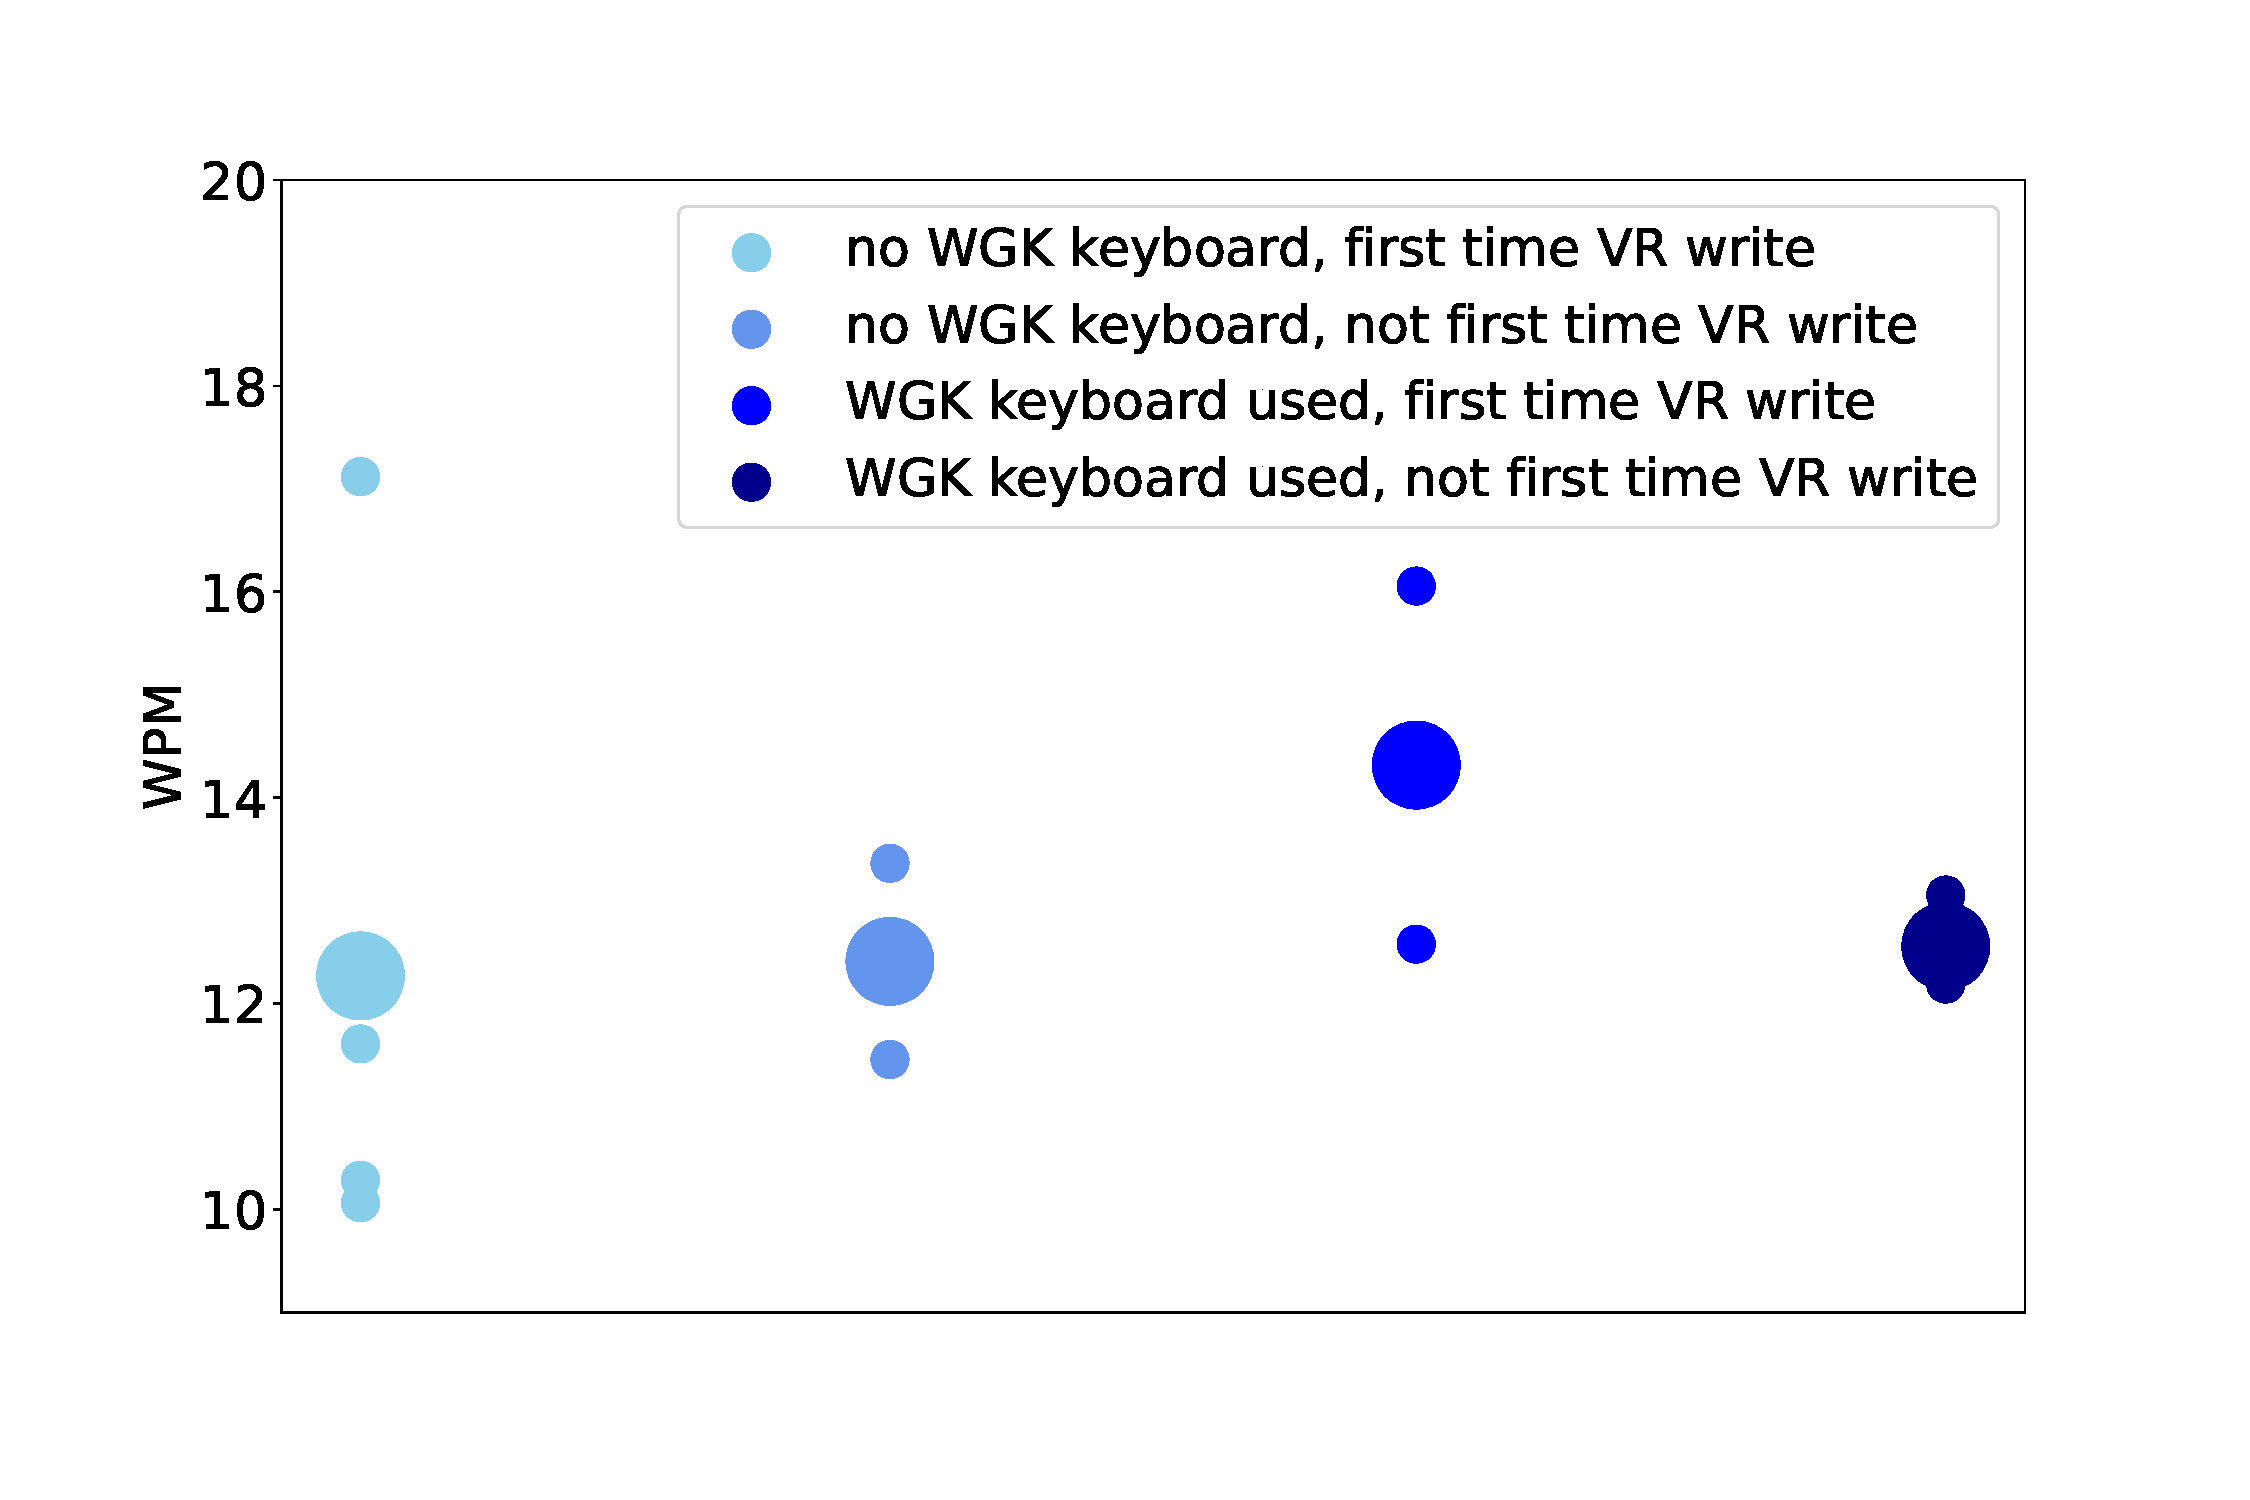
\includegraphics[width=0.9\textwidth]{Comparison_yesno.pdf}
    \caption{Each small dot shows the average WPM for a user. The big dots represent the average WPM per group. The colors are for the different groups of experience in VR writing and word-gesture keyboards}
    \label{fig:WPM_yesno}
\end{figure}
In Fig \ref{fig:WPM_yesno} we can see that against our predictions the prior knowledge some participants have, did not really help them to write faster. In fact, the fastest group was the one that is experienced with word-gesture keyboards but not with writing in VR. We can also observe that the participant with the highest average WPM is in the group that has no experience with any of these two things. But we think these results might not be too representative due to the small sizes of the groups.\\

Another thing we analyze is the writing speed compared to the age.
\begin{figure}[H]
    \centering
    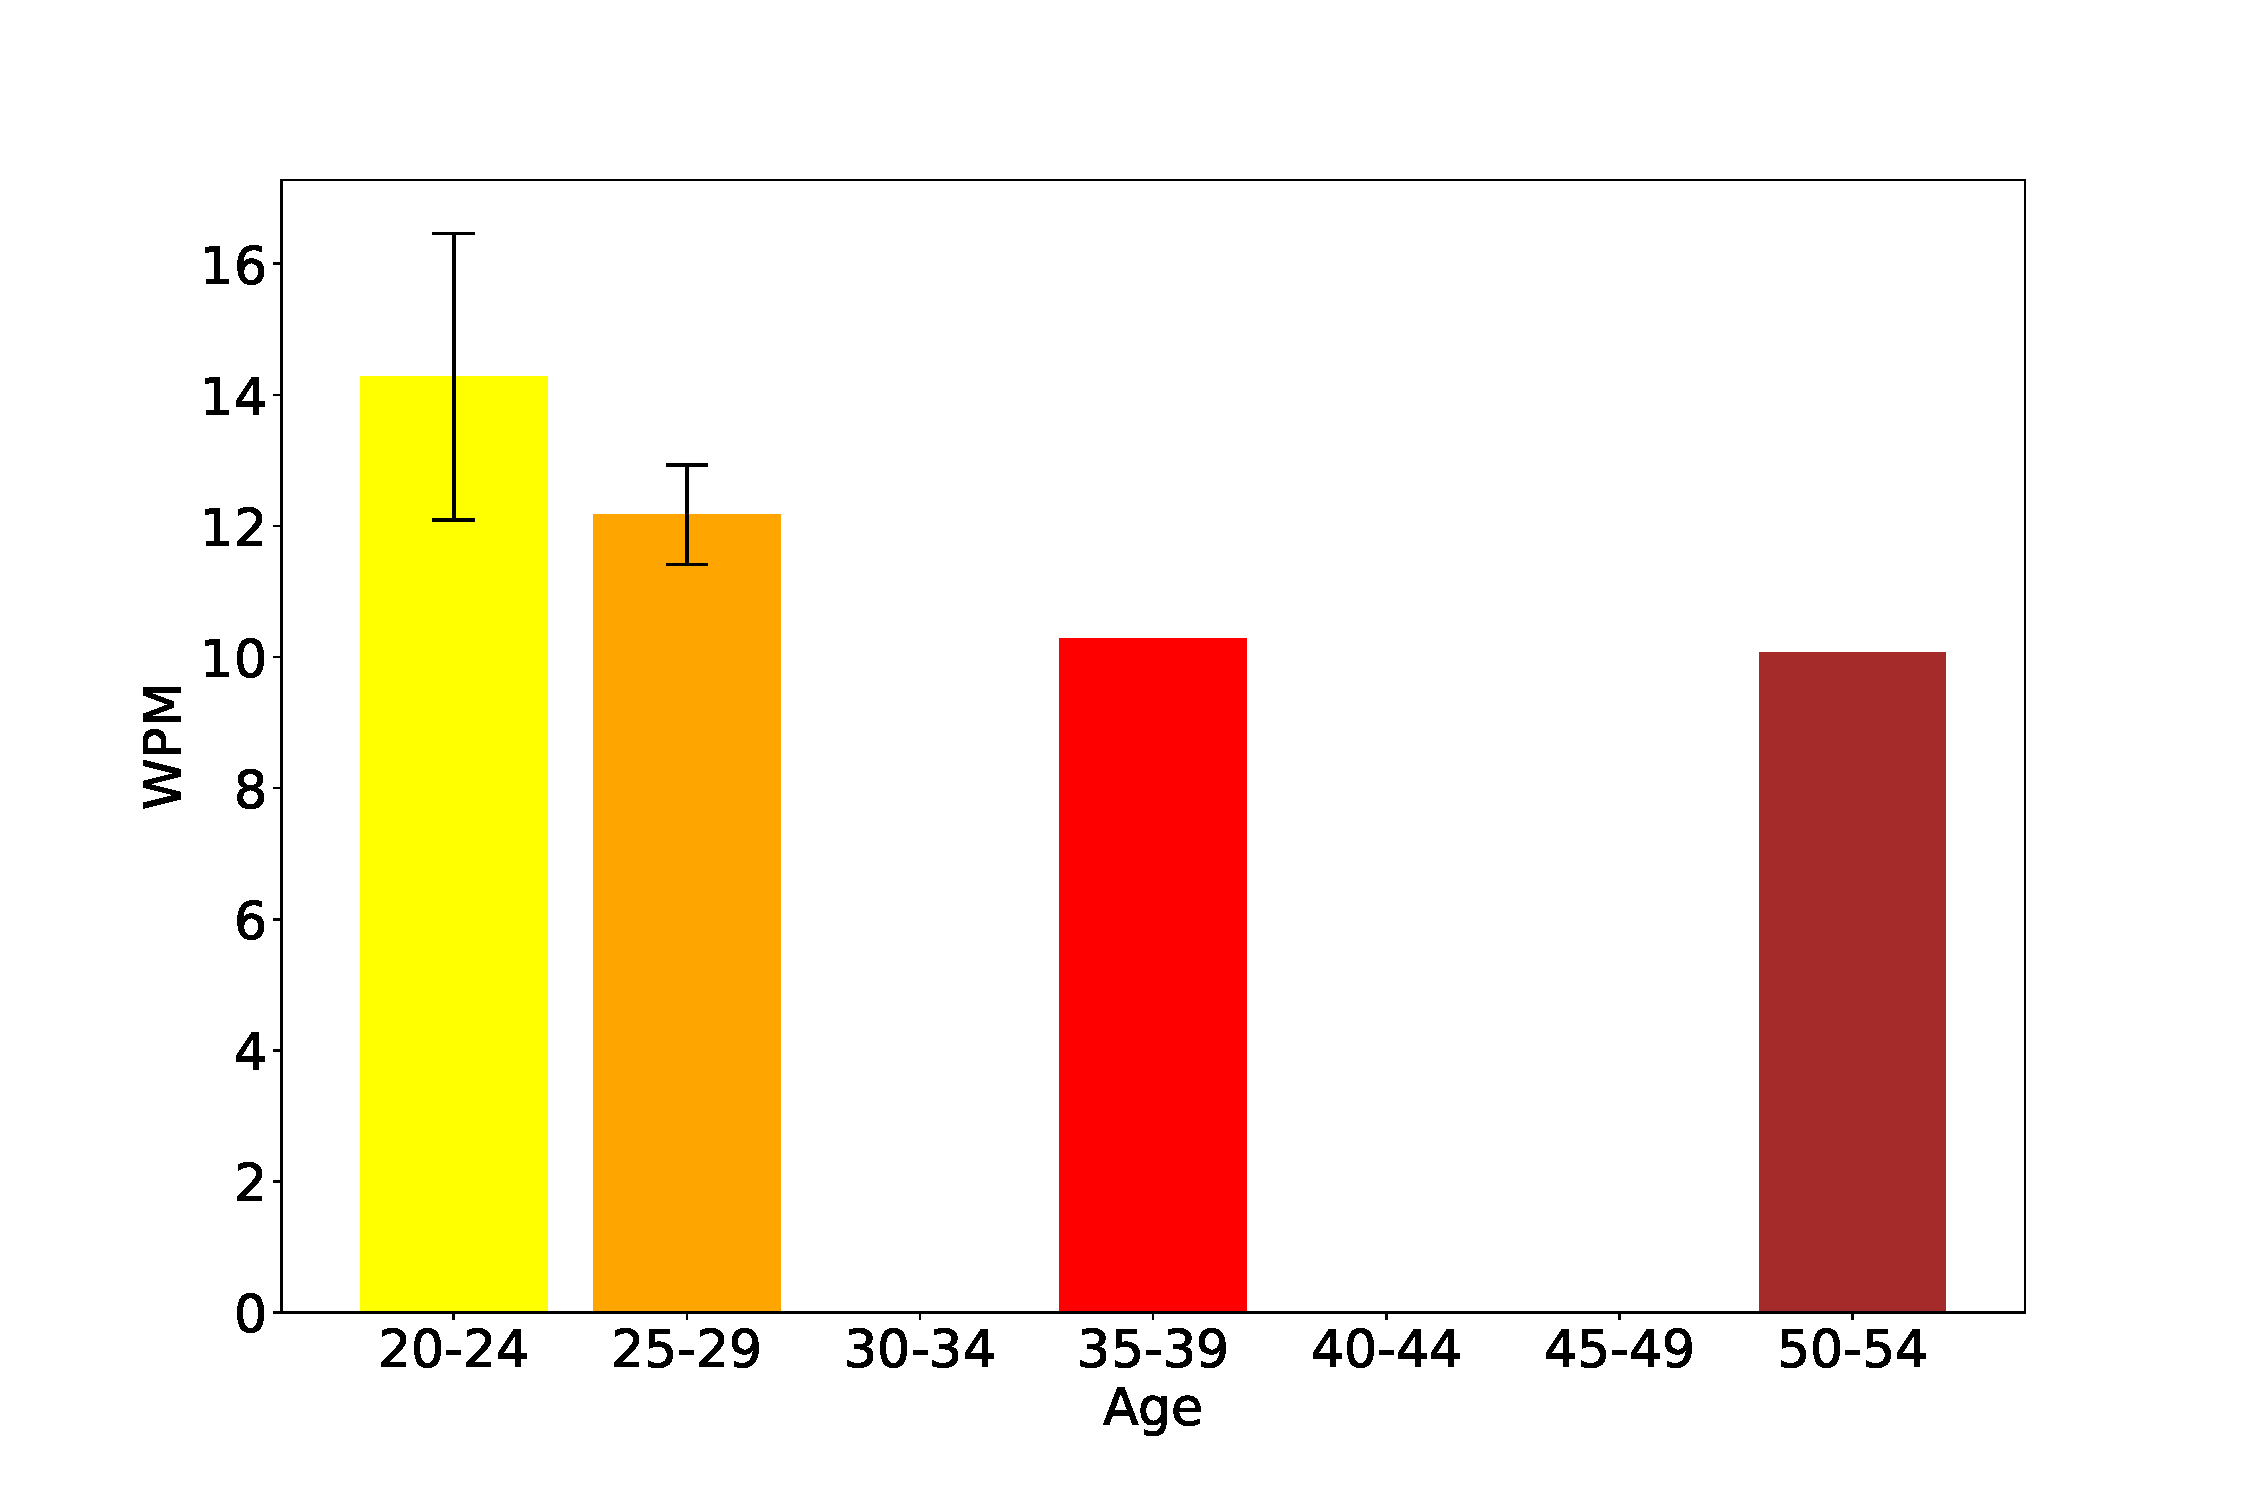
\includegraphics[width=0.9\textwidth]{age_wpm.pdf}
    \caption{WPM values sorted by age groups of five years. The 20-24 and 25-29 groups also have a standard deviation error bar, because they consist of five and four participants. The 35-39 and 50-54 groups do not have an error bar since each of them only contains of one participant.}
    \label{fig:WPM_age}
\end{figure}

We might expect that older people are a bit slower in writing in VR than younger ones. Actually, this is what we can observe in Fig \ref{fig:WPM_age}. At least among our participants, the WPM value decreases with the increase in age. This means, the older participants were a bit slower than the younger ones. But again, due to the low amount of participants in the older age groups, the results are not too representative and must be viewed with caution.\\

To end this section about writing speed, we check what is the fastest possible WPM we could reach. Zhai and Kristensson \cite{Kristensson2004SHARK2AL} made this experiment with four different phrases. We take the same phrases and compare their results with the ones we get. The four phrases are:\\
1. The quick brown fox jumps over the lazy dog\\
2. Ask not what your country can do for you\\
3. East west north south\\
4. Up down left right\\

\begin{table}[H]
    \centering
    \caption{Fastest achieved WPM value per sentence for each person}
    \begin{tabular}{cccc} \toprule
        Phrase&$\text{SHARK}^2$ Author A&$\text{SHARK}^2$ Author B&Author of this work\\ \midrule
        1&69.0&70.3&47.78\\
        2&51.6&60.0&48.48\\
        3&74.4&72.9&70.22\\
        4&74.1&85.6&58.04\\
        \bottomrule
    \end{tabular}
    \label{tab:top speed}
\end{table}
We can see that we can not reach the same maximal WPM but especially for phrase 3 we can get close to their value. The word-gesture keyboard is obviously faster if it is on a small screen and a finger is used. The distances that have to be covered are much smaller than in VR, hence it makes it easier to write fast. Nevertheless, we think we still reached a high WPM value.

\subsection{Error Rate}
In this section, we will look at different error rates. First of all, we want to find out, which words caused most of the errors. Later, we will examine different errors caused by the participants.

\subsubsection{Most Common Error Words}
We look at all the words that were not the best match. We do not differentiate between the ones that were in the keyboard suggestions and the ones that were not. We call such a word ``error word''. The top ten such words are listed in the following table:
\begin{table}[H]
    \centering
    \caption{Most common words that were not the best match in the evaluation.}
    \begin{tabular}{cc} \toprule
        word&times wrong\\ \midrule
        the & 53\\
        is & 17\\
        to & 14\\
        of & 12\\
        in & 9\\
        for & 8\\
        do & 5\\
        all & 3\\
        more & 3\\
        see & 2\\
        \bottomrule
    \end{tabular}
    \label{tab:error_words}
\end{table}

As we can see in Table \ref{tab:error_words}, the most common error word is ``the'', which has a count of 53. In this list, we can also see other words whose errors could be avoided by a better implementation of the word detecting algorithm. For example ``in'' and ``more'' are such words. The best match, when a participant wanted to write these words, were ``thee'', ``inn'' and ``moore'', which are words that do not appear that much in plain language. For other words like ``to'' or ``of'', whose best matches were ``too'' or ``off'', it is maybe not as easy to get the right word because all of them appear fairly often in plain language.

\subsubsection{Backspace Error Rate}
The erroneous keystroke error rate (EKS ER) \cite{ArifTextEntry} measures the ratio of the total number of erroneous keystrokes to the length of the phrase that has to be written. In another paper, Chen et al. \cite{10.1145/3290607.3312762} use a metric derived from the EKS ER. Instead of the erroneous keystrokes, they take the number of times the backspace key was used. For our calculations, we will use the same metric as they do. We call this the ``backspace error rate'' and calculate it with following formula:
\begin{equation}
    \text{backspace error rate} = \frac{\text{\#backspaces used}}{\mid P \mid} \times 100\%
\end{equation}
where $\mid P \mid$ is the number of characters a participant had to write.
\iffalse
\begin{figure}[H]
    \centering
    \makebox[\textwidth][c]{
        \centering
        \subbottom[backspace error rate compared to WPM\label{fig:error_backspace:error_backspace1}]{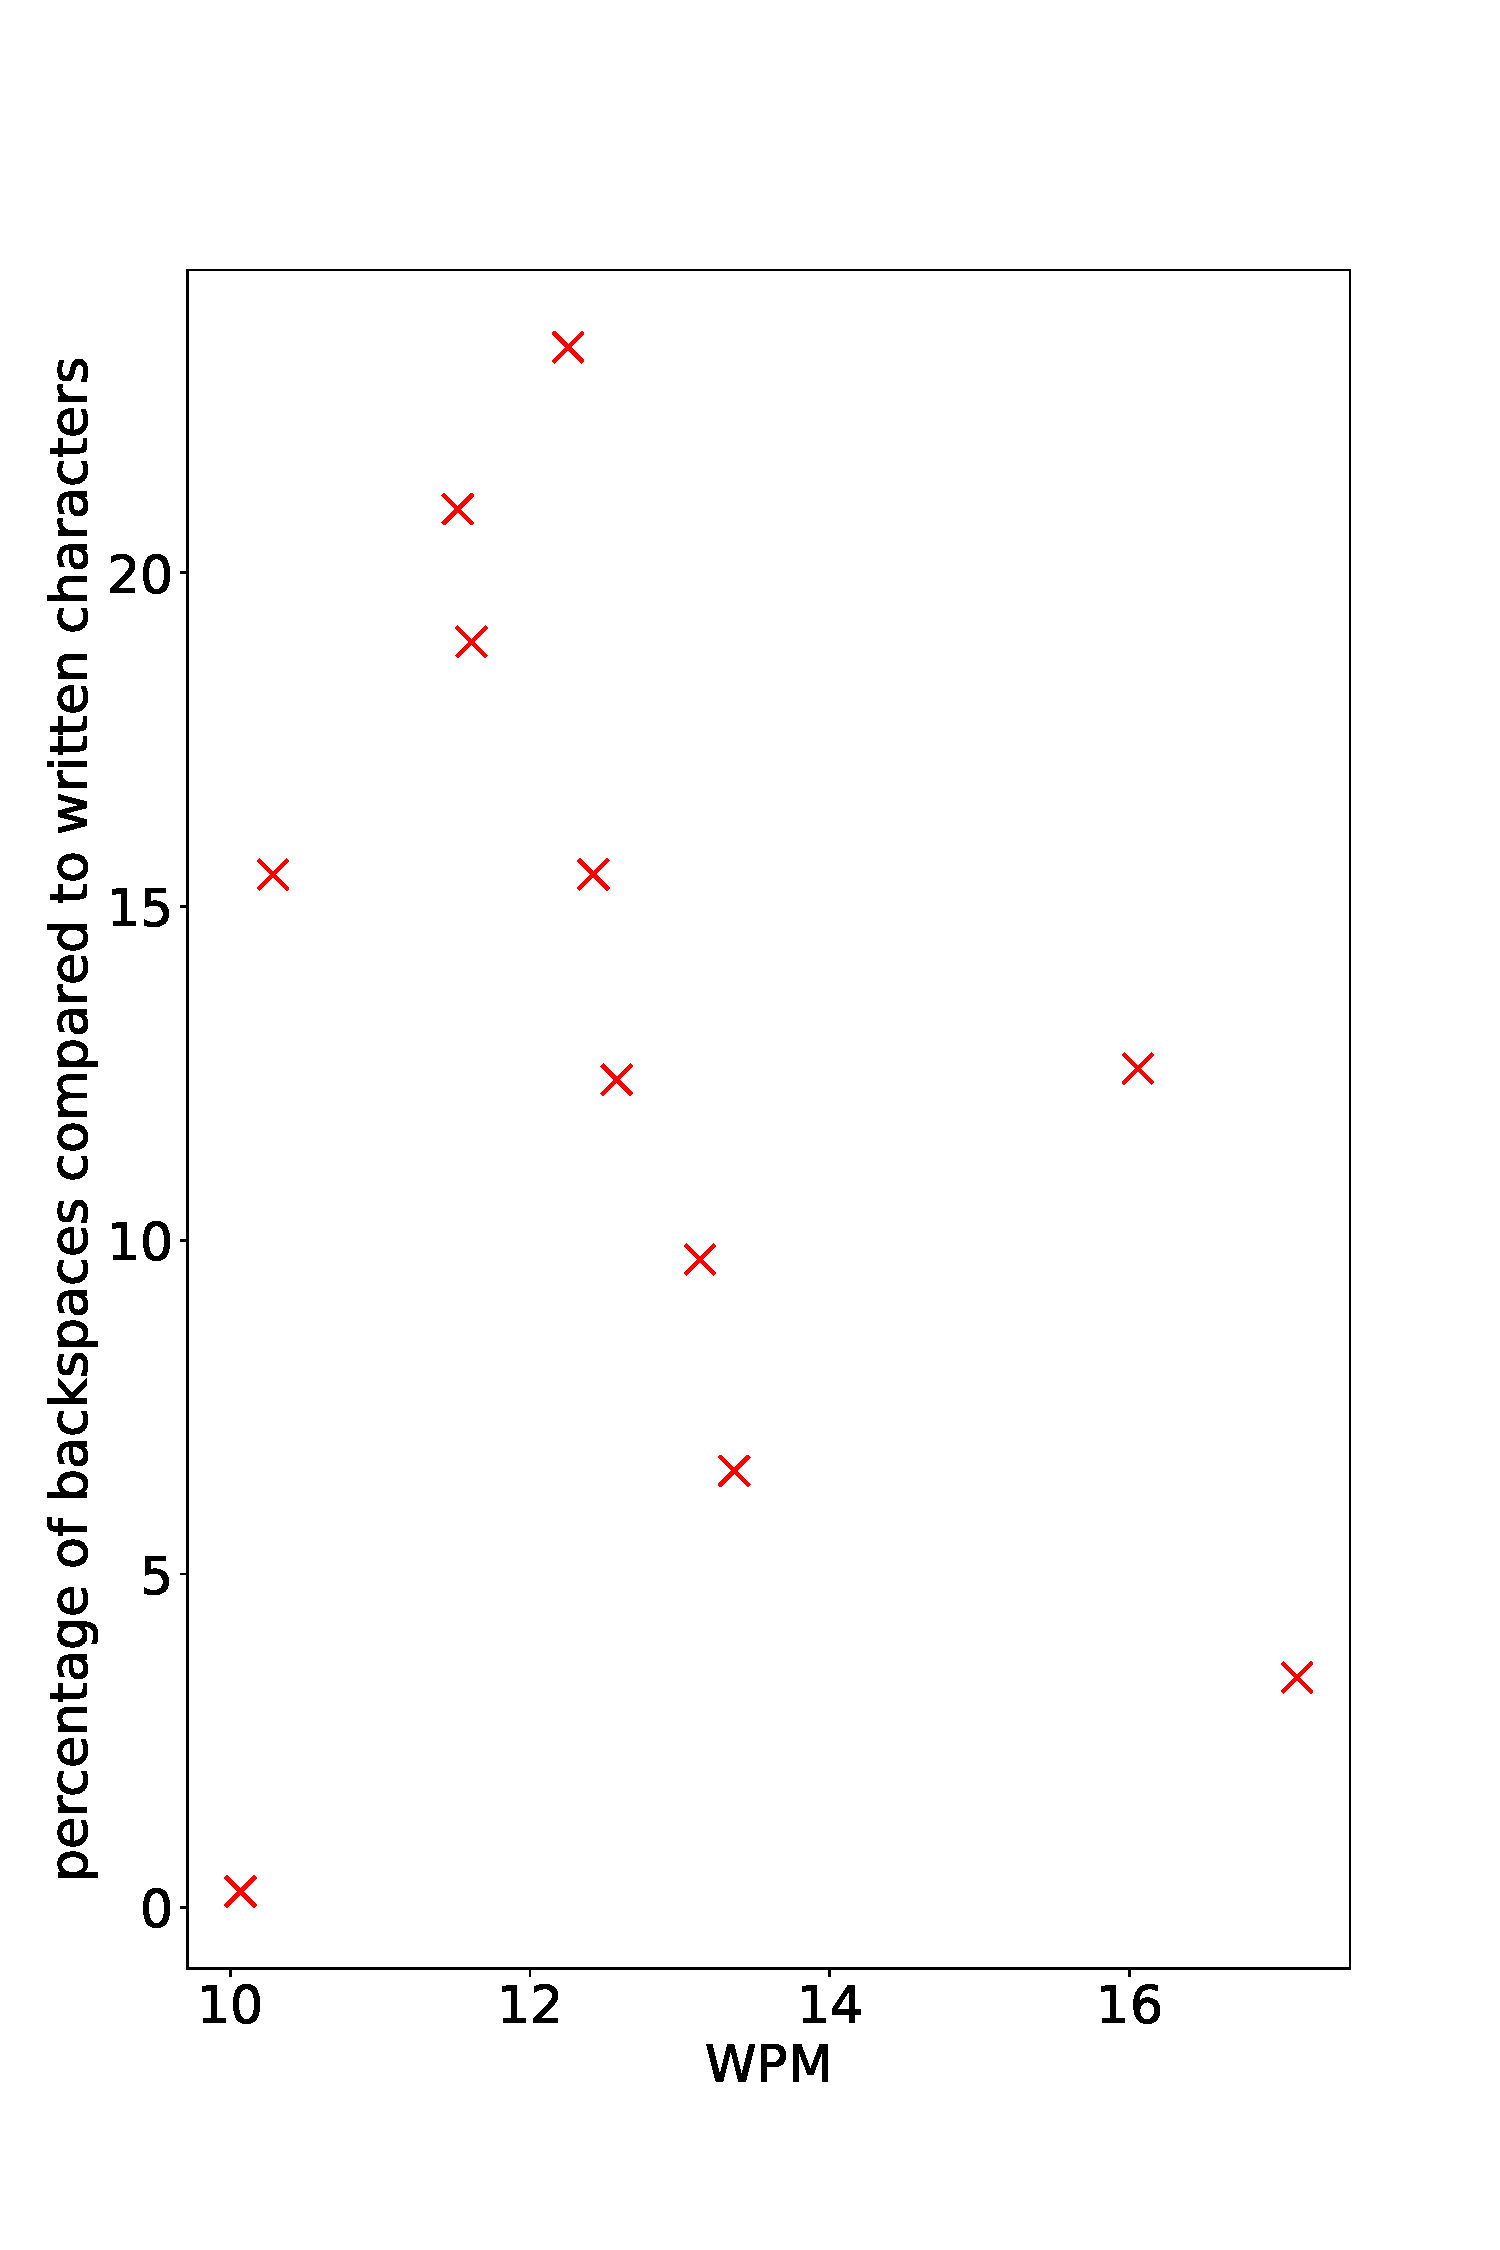
\includegraphics[width=0.6\textwidth]{backspace_error2.pdf}}\hspace{-3.0em}
        \subbottom[a boxplot for the backspace error rate over all participants. The orange line is for the median, the rectangle shows the 25\% and 75\% quartiles, and the upper and lower whiskers show the maximum and minimum.
        \vspace{-3em}
        \label{fig:error_backspace:error_backspace2}]{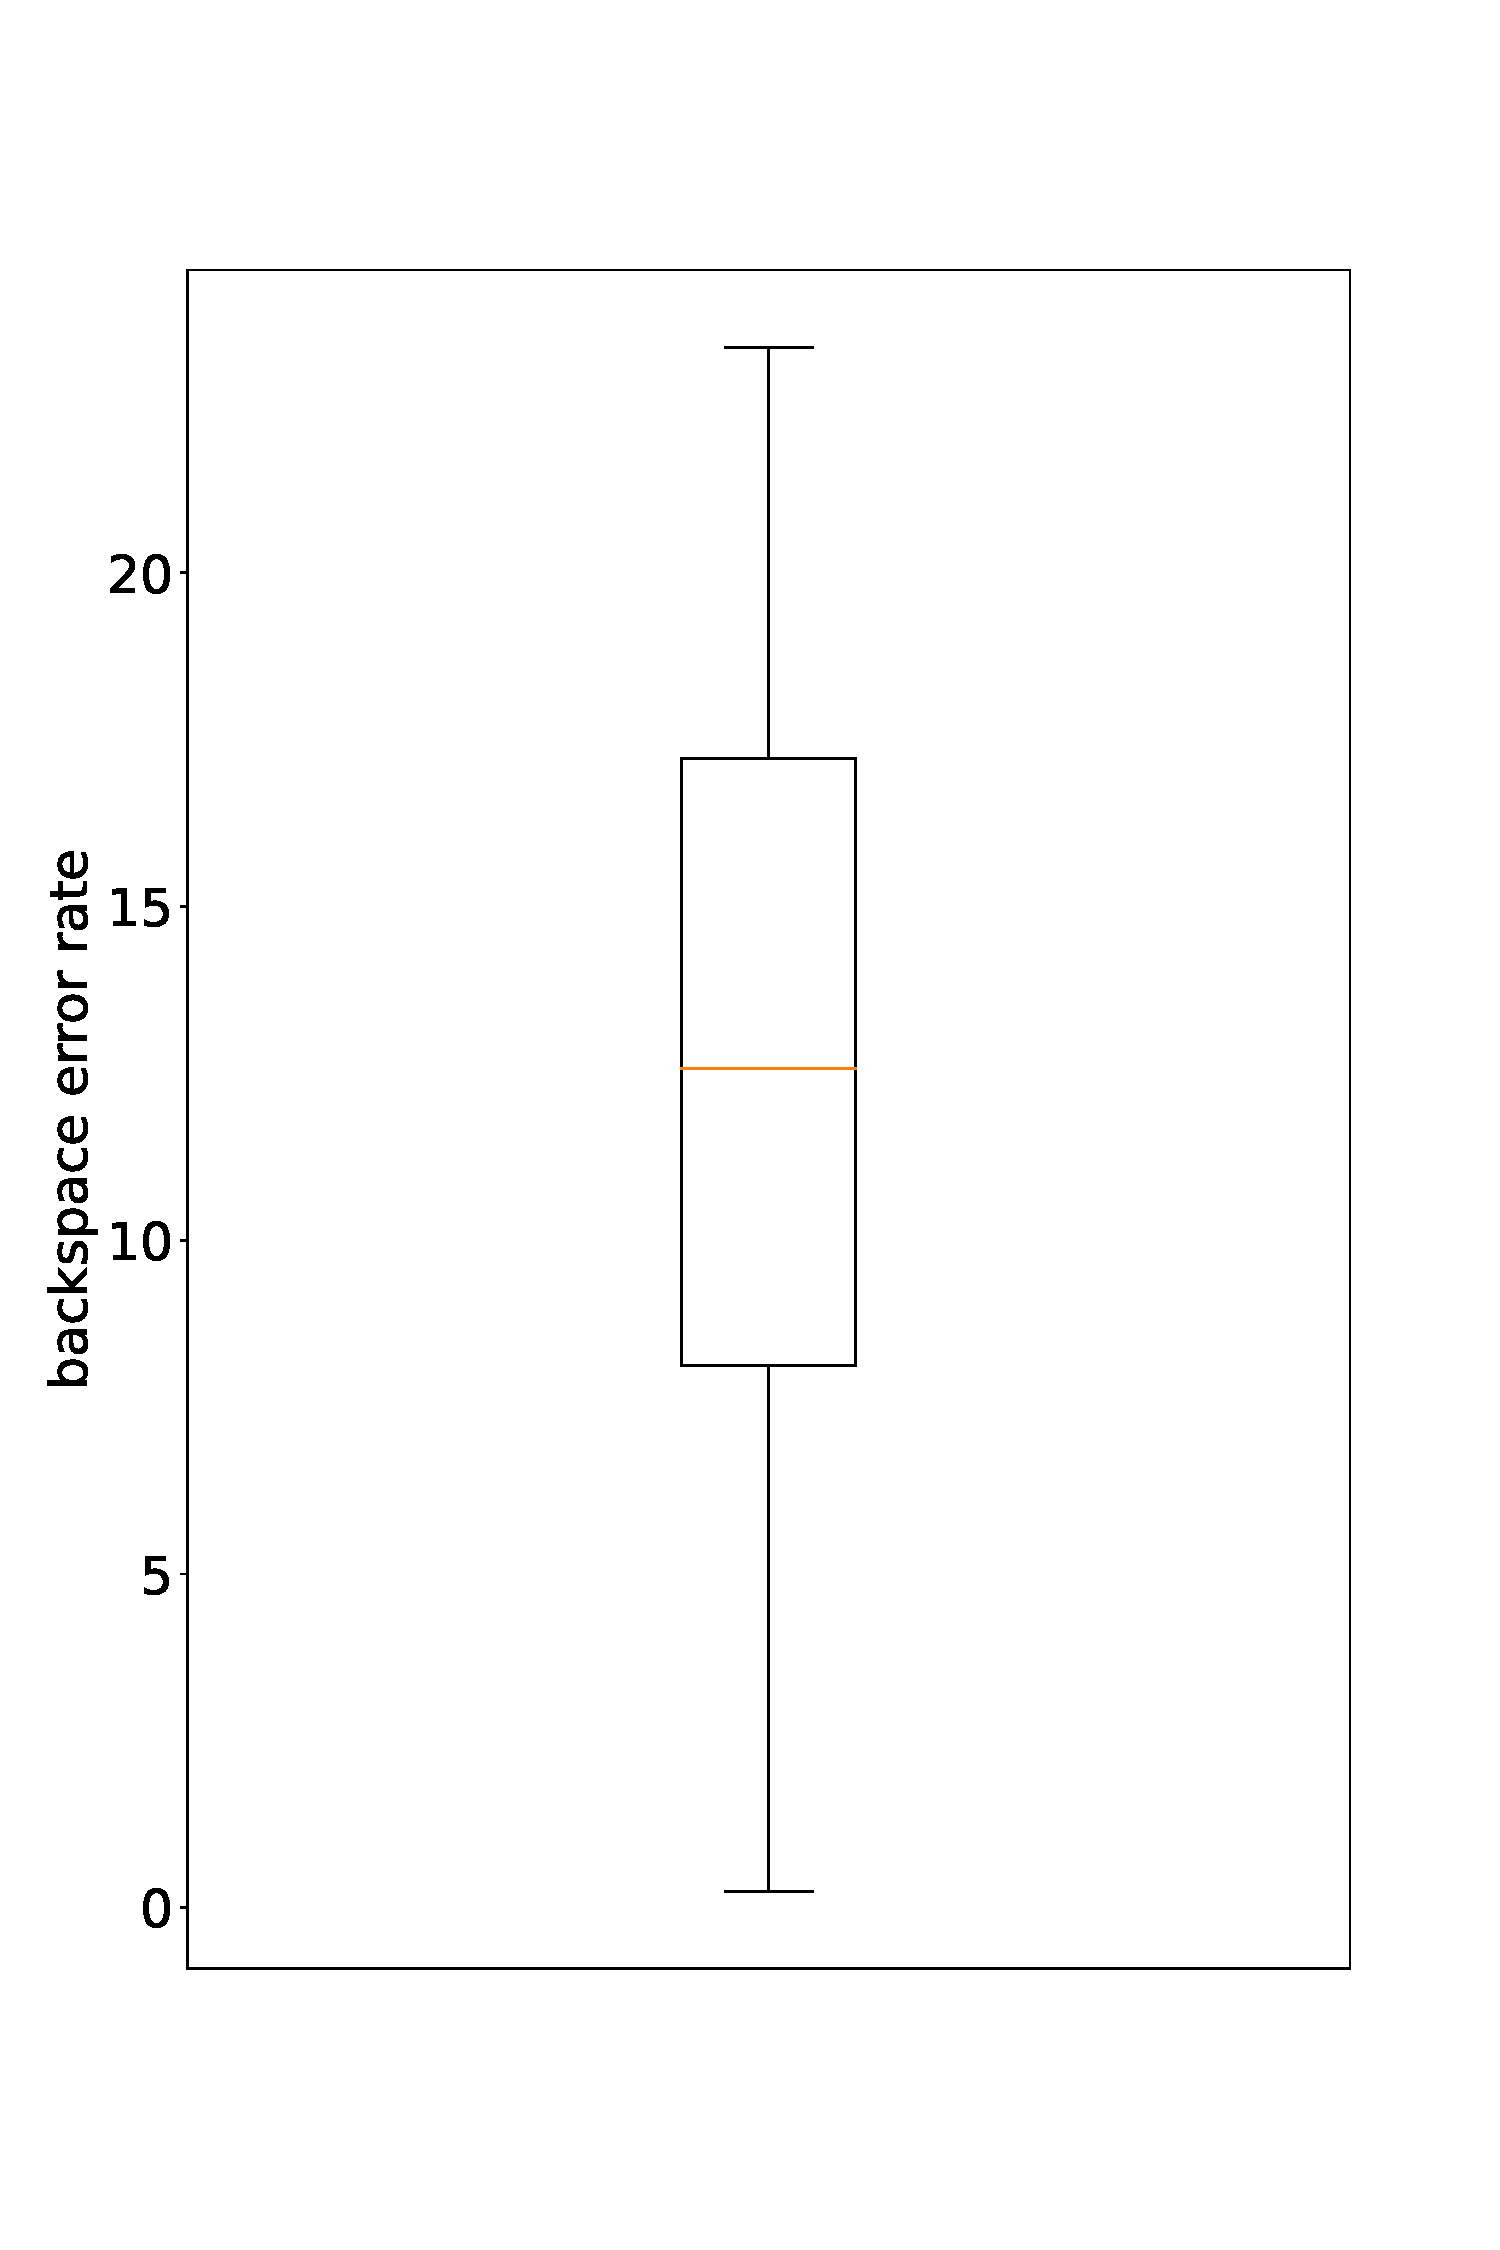
\includegraphics[width=0.6\textwidth]{ekser_boxplot.pdf}}
    }
    \vspace{2em}
    \caption{shows the backspace error rate in two different ways. (a) with a comparison to the WPM of each participant and (b) a boxplot combining all participants' backspace error values.}
    \label{fig:error_backspace}
\end{figure}
\fi
\begin{table}[H]
    \centering
    \caption{Backspace error rate per participant and average over all}
    \begin{tabular}{cc} \toprule
        Participant&Backspace ER\\ \midrule
        1 & 20.95\%\\
        2 & 23.38\%\\
        3 & 9.71\%\\
        4 & 18.97\%\\
        5 & 12.40\%\\
        6 & 15.48\%\\
        7 & 15.48\%\\
        8 & 12.57\%\\
        9 & 6.54\%\\
        10 & 3.45\%\\
        11 & 0.24\%\\
        \midrule
        average & 12.65\%\\
        \bottomrule
    \end{tabular}
    \label{tab:backspace_er}
\end{table}
In \Cref{tab:backspace_er} the average backspace error rate of 12.65\% is listed. This means, for every input of 100 correct characters about 13 backspaces were used. Again, as for the WPM previously, we compare our calculated backspace error rate with another existing work. As mentioned above, we calculate the same metric as Chen et al. did in their work \cite{10.1145/3290607.3312762}. Therefore, we compare it to their results:
\begin{table}[H]
    \centering
    \caption{Comparison of backspace error rates}
    \begin{tabular}{cc} \toprule
        text input method&backspace error rate\\ \midrule
        Word-gesture keyboard raycasting&15.64\%\\
        Our word-gesture keyboard&12.65\%\\
        \bottomrule
    \end{tabular}
    \label{tab:error_backspace_compare}
\end{table}
In \Cref{tab:error_backspace_compare} we can see that the error values are pretty much the same, although our value is a bit better. A reason for this might be that they did not implement that a word can be deleted as a whole. For example, if the newest written word is wrong the user can just press the backspace key once and delete the whole word when using our system. Now, they possibly implemented that no matter the last input every character must be deleted individually, which would result in more needed backspaces.

\subsubsection{Total ER}
\label{sec:total_er}
The next error rate we calculate is the Total ER according to Soukoreff and MacKenzie \cite{10.1145/642611.642632}. For this we use following formula:

\begin{equation}
    Total\ ER = \frac{INF + IF}{C + INF + IF} \times 100\%
\end{equation}

where $C$ is the number of correct characters in the transcribed text. The transcribed text consists of all phrases a participant ``sends'' before beginning with a new one. Next, $INF$ denotes the minimum string distance between the transcribed text and the given phrases. The MSD value is the number of single character insertions, deletions or substitutions to get from the wrong string to the right one. For example, to get from ``thee'' to ``the'', we need one deletion, therefore the MSD value would be 1. Finally, $IF$ denotes the keystrokes in the input stream (everything a participant inputted during their evaluation) that are not in the transcribed text and not editing keys.\\
In our evaluation, a participant could only go to the next phrase if they inputted the last one correctly without any mistake. This means $C$ is the number of characters a participant had to write and $INF$ is 0. It is 0 because, as mentioned right before, the transcribed text had to equal the text they had to write. So, these two values are taken as mentioned in \cite{10.1145/642611.642632}. However, for $IF$ we have to use a bit another value as specified. Due to lacking evaluation records, we do not have the full input stream. Therefore, we can not just count the characters that were written too much. Soukoreff and MacKenzie also mention a fourth value $F$ that counts the number of editing keys (backspaces, delete, ...) used. They mention that $F = IF$. Therefore, we will assign $F$ the number of backspaces used and set $IF$ equal to $F$. Important to mention is that if counted correctly $IF$ would be a bit larger because if one backspace is used, sometimes a whole word gets deleted. But this should not have happened too many times. Most of the time the user needed the backspace to delete a whole word only after writing a wrong word with the correct word not being in the suggestions. Otherwise, they deleted single characters. This means it is not a bad approximation of the real $IF$ value.
\begin{table}[H]
    \centering
    \caption{Total ER per participant and average over all}
    \begin{tabular}{cr} \toprule
        participant&total ER\\ \midrule
        1&17.32\%\\
        2&18.95\%\\
        3&8.85\%\\
        4&15.94\%\\
        5&11.03\%\\
        6&13.40\%\\
        7&13.41\%\\
        8&11.17\%\\
        9&6.14\%\\
        10&3.33\%\\
        11&0.24\%\\\midrule
        average&10.89\%\\
        \bottomrule
    \end{tabular}
    \label{tab:total_er}
\end{table}
As we can see in Table \ref{tab:total_er}, the averge is 10.89\% with a standard deviation of 5.57. We can not really say if this is a high error rate or rather a low one. Therefore, we make another comparison with the results of Boletsis and Kongsvik \cite{Boletsis2019ControllerbasedTT}:
\begin{table}[H]
    \centering
    \caption{Comparison of the total ER for different VR text input methods}
    \begin{tabular}{lr} \toprule
        text input method&total ER\\ \midrule
        Split keyboard& 8.11\%\\
        Head-directed input keyboard& 10.15\%\\
        \textbf{Word-gesture keyboard (ours)}& 10.89\%\\
        Raycasting keyboard& 11.05\%\\
        Drum-like keyboard& 12.11\%\\
        \bottomrule
    \end{tabular}
    \label{tab:total_er_compare}
\end{table}
The total ER for our keyboard seems also to be ranked in the middle as the WPM value before. An explanation for this could be that we forced the participants to correct errors because they could only continue with the next phrase, if the last one was correct. Thus, a lot of participants saw an error only when they thought they had ended a phrase. Then, they had to delete half of the phrase to be able to correct the error. Boletsis and Kongsvik \cite{Boletsis2019ControllerbasedTT} on the other did allow transcribed texts that are not correct. If we had also done this, the $IF$ value would be much lower. Obviously the $INF$ value would increase but not as much as $IF$ would decrease. While to the $INF$ value only some characters would be added from wrong words in the transcribed text, the $IF$ value would sometimes be only a fraction of itself because participant would not have deleted half of a phrase as many times as they did now. This means that our total ER value could be lowered if we had taken another evaluation approach. Nevertheless, it is still not bad as it is right now.

\subsubsection{Participant Conscientiousness}TODO EVTL REMOVE TOTAL ER REFERENCE
For the next calculation, we investigate the percentage of not immediately corrected words. Not immediately corrected (NIC) words are the ones, where the best match is not the intended word and the word would be in the keyboard's word suggestions, but the participant does not choose it. Firstly, we will do this with characters and then with the whole words. For the calculation with the characters of a NIC word we take the MSD values as we did in the previous calculation with the total ER. Then we want to compare these two values with the same approach, but without considering the errors happened because of ``the'', ``in'' and ``more''. We decide to remove these three words because they could be avoided by a small change in the best match calculations, and we are interested, if there are any differences worth mentioning.
\iffalse
\begin{figure}[H]
    \makebox[\textwidth][c]{
        \centering
        \subbottom[Not corrected characters with WPM\label{fig:error_user:error_user1}]{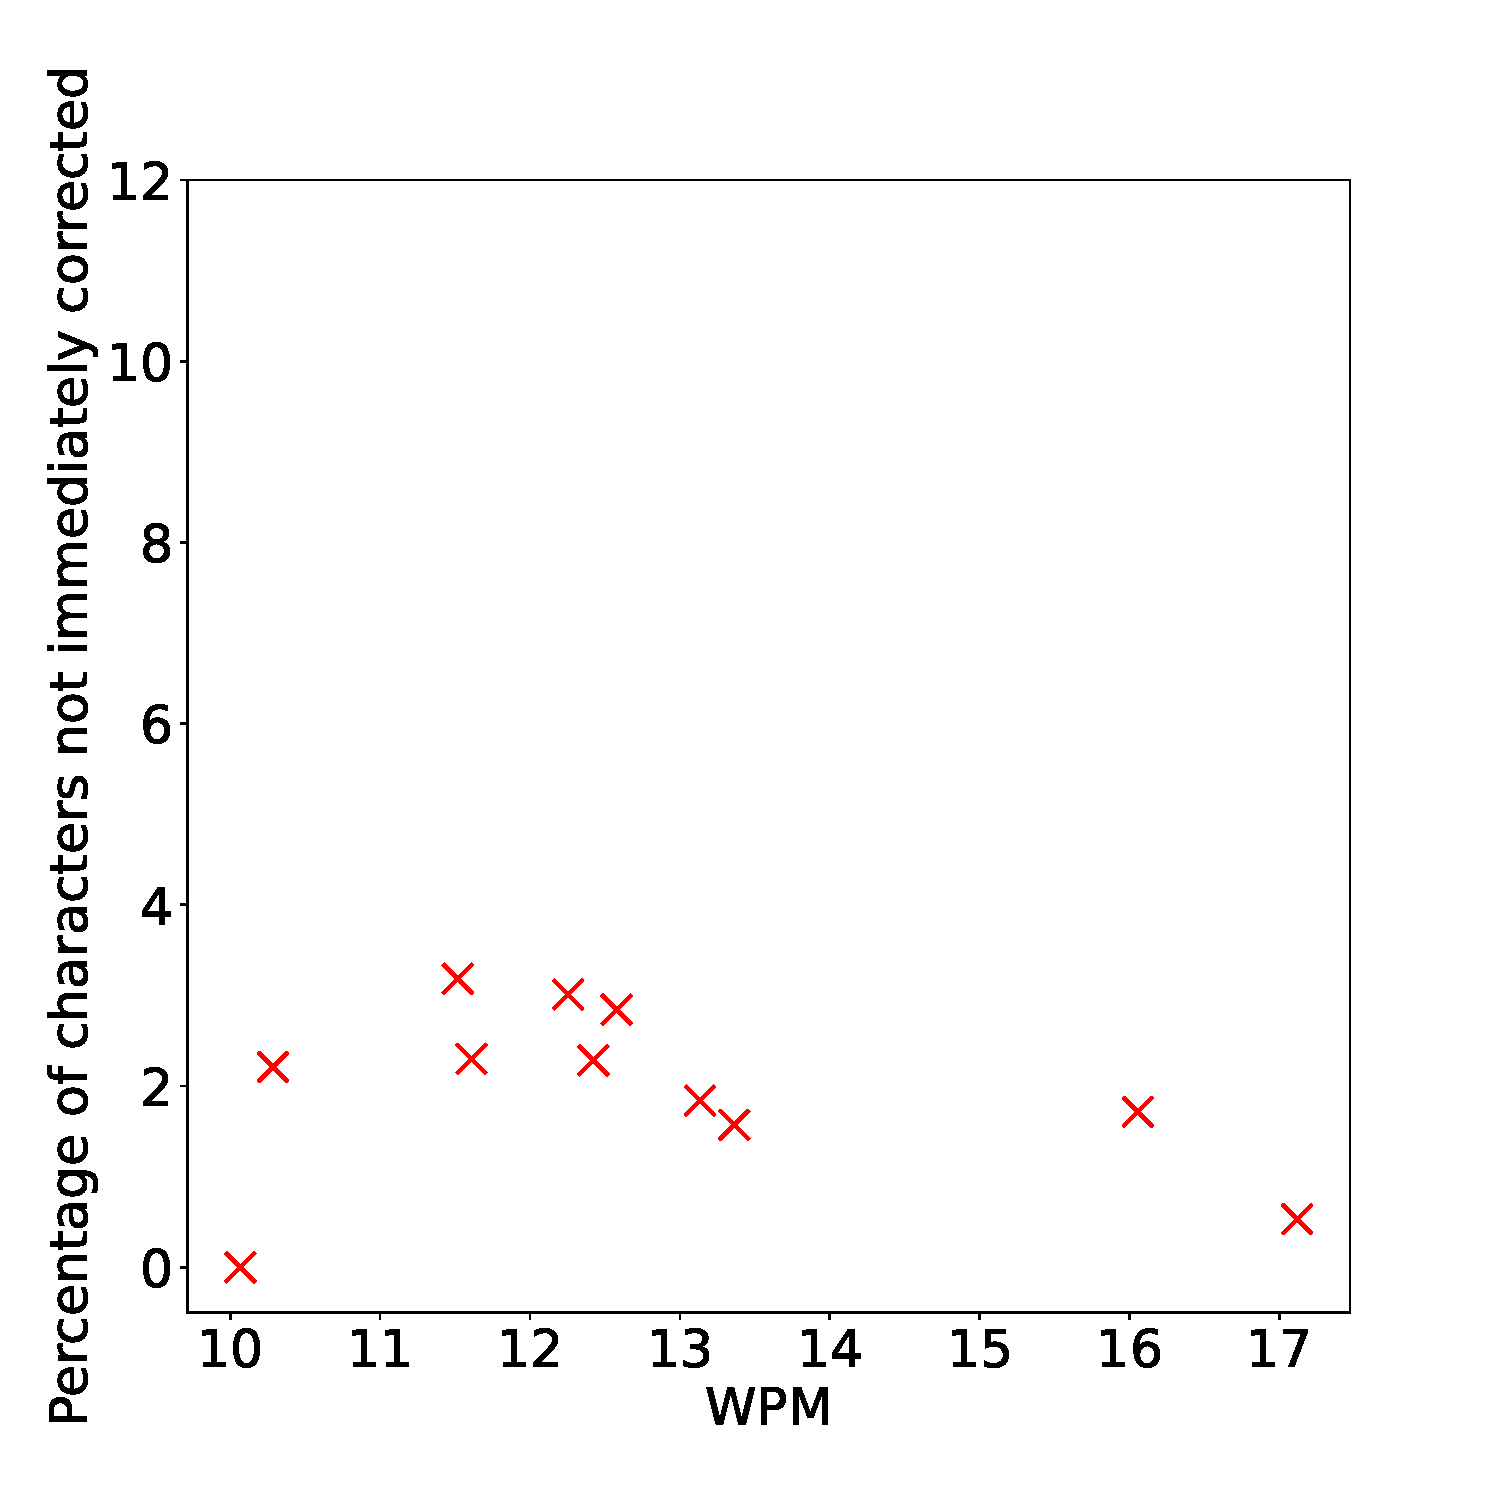
\includegraphics[width=0.6\textwidth]{user_error3_1.pdf}}\hspace{-3.0em}
        \subbottom[As (a), but without ``the'', ``in'' and ``more''\label{fig:error_user:error_user2}]{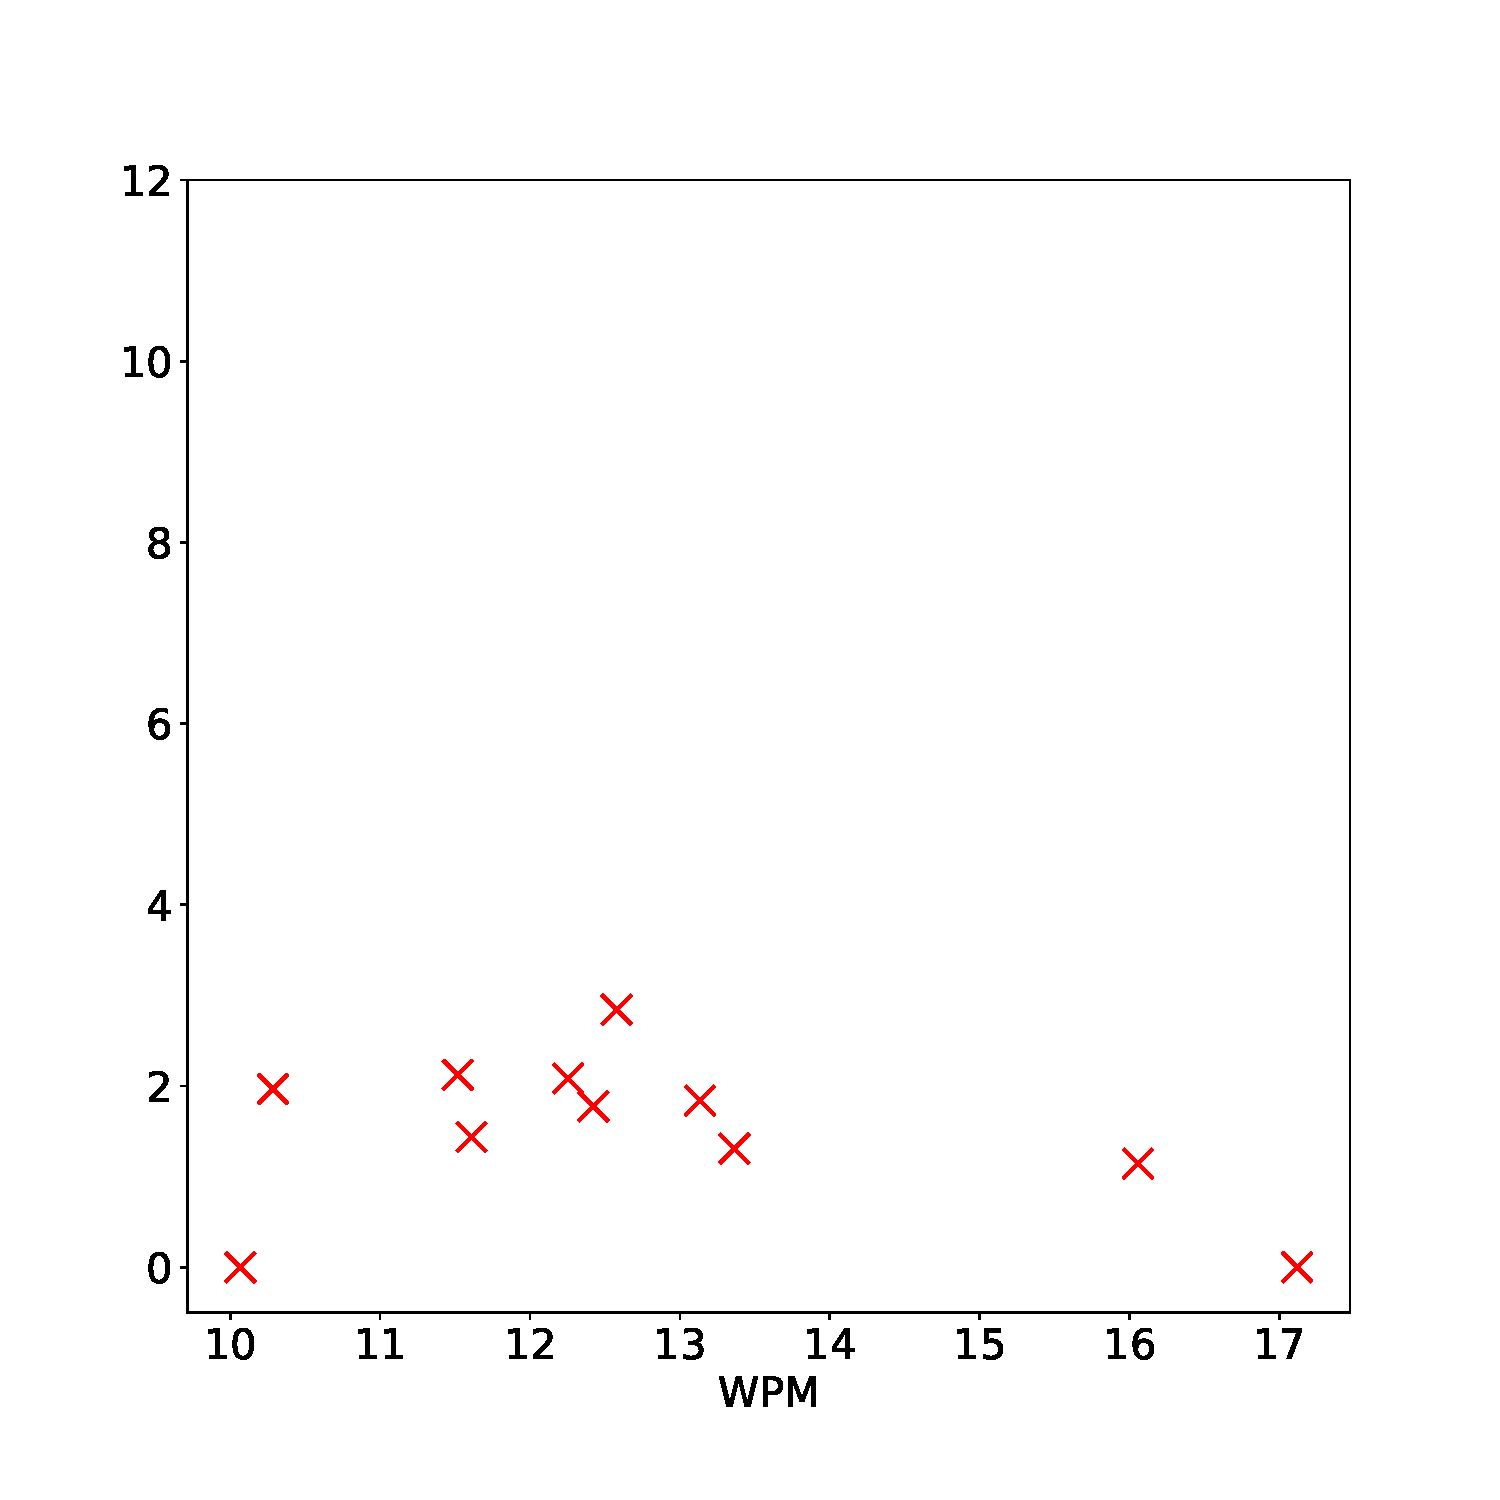
\includegraphics[width=0.6\textwidth]{user_error3_2.pdf}}
    }
    \makebox[\textwidth][c]{
        \centering
        \subbottom[Not corrected words with WPM\label{fig:error_user:error_user3}]{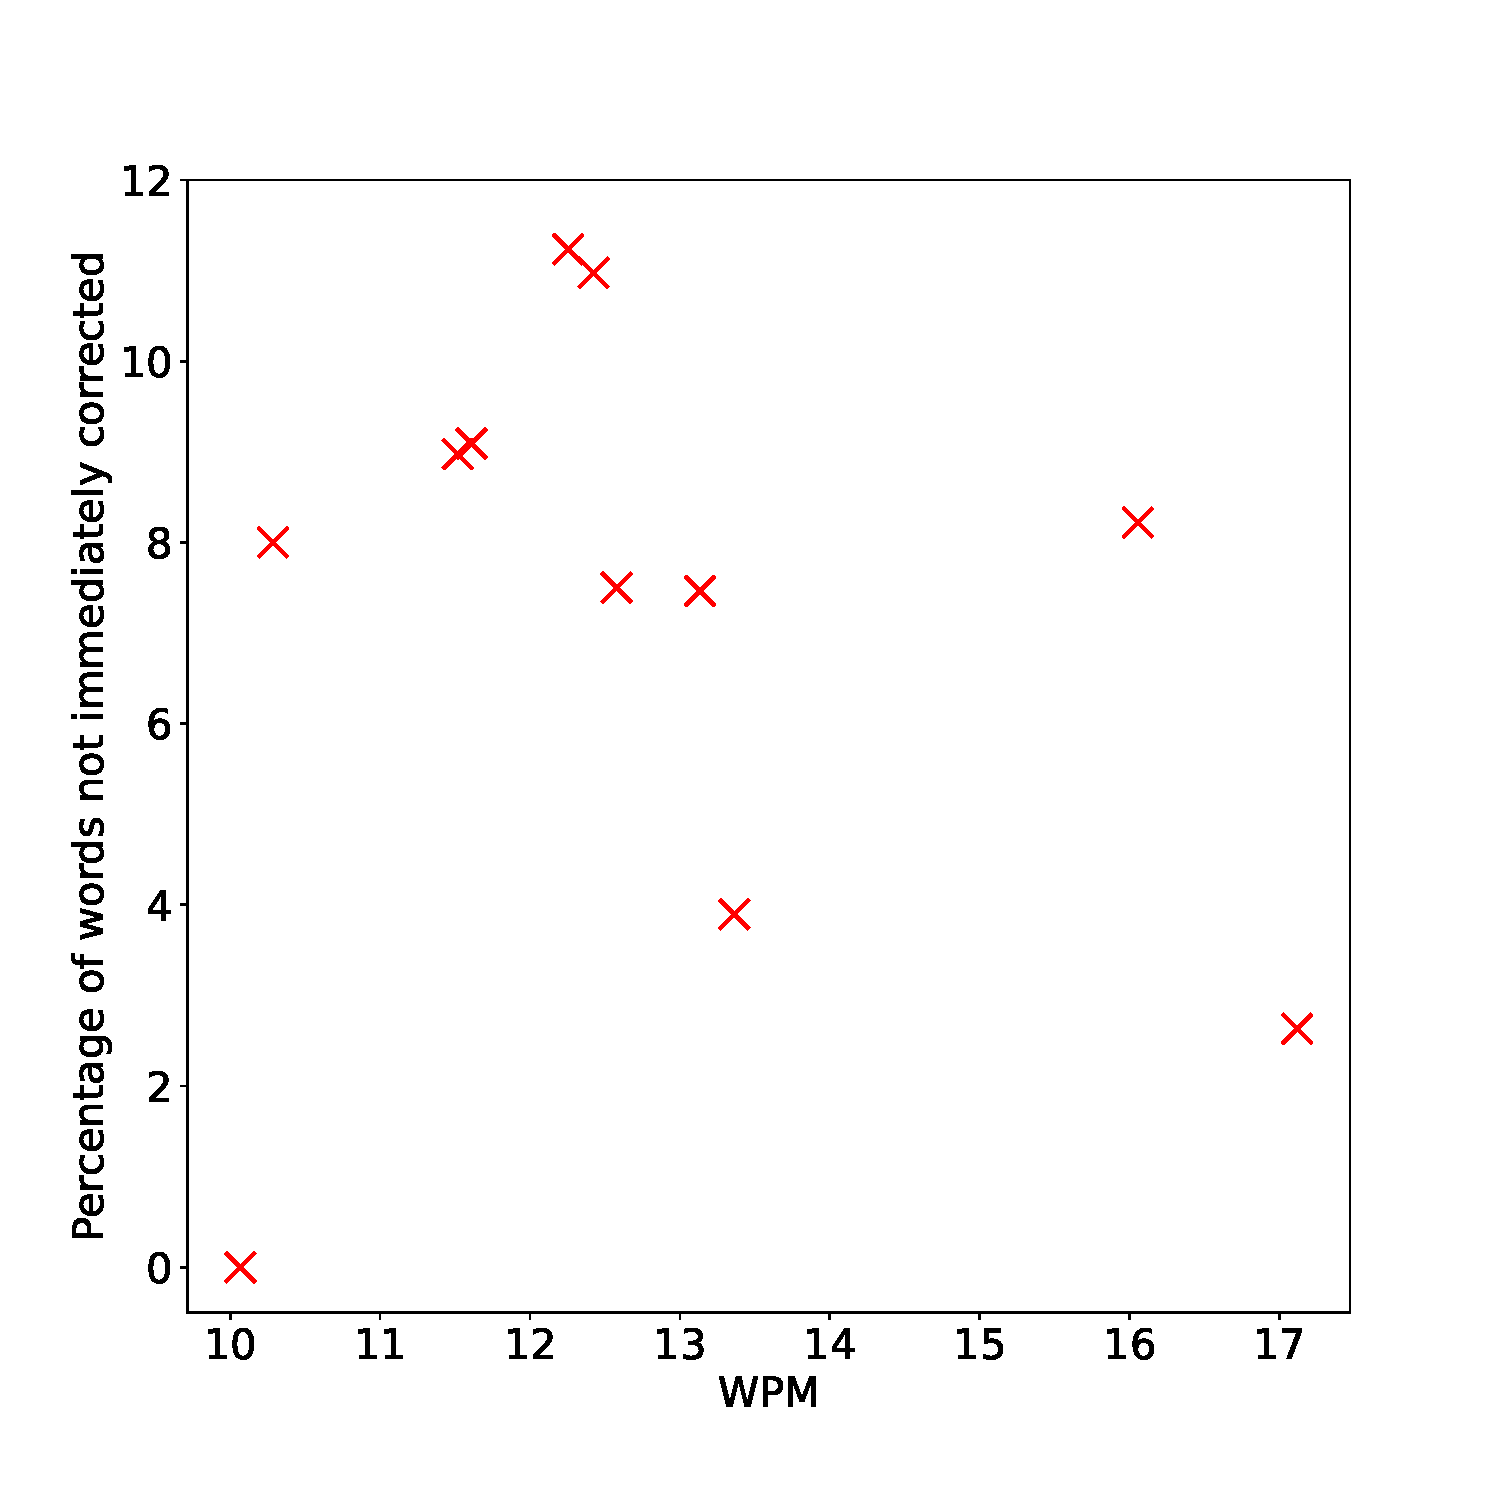
\includegraphics[width=0.6\textwidth]{user_error3_3.pdf}}\hspace{-3.0em}
        \subbottom[As (c), but without ``the'', ``in'' and ``more''\label{fig:error_user:error_user4}]{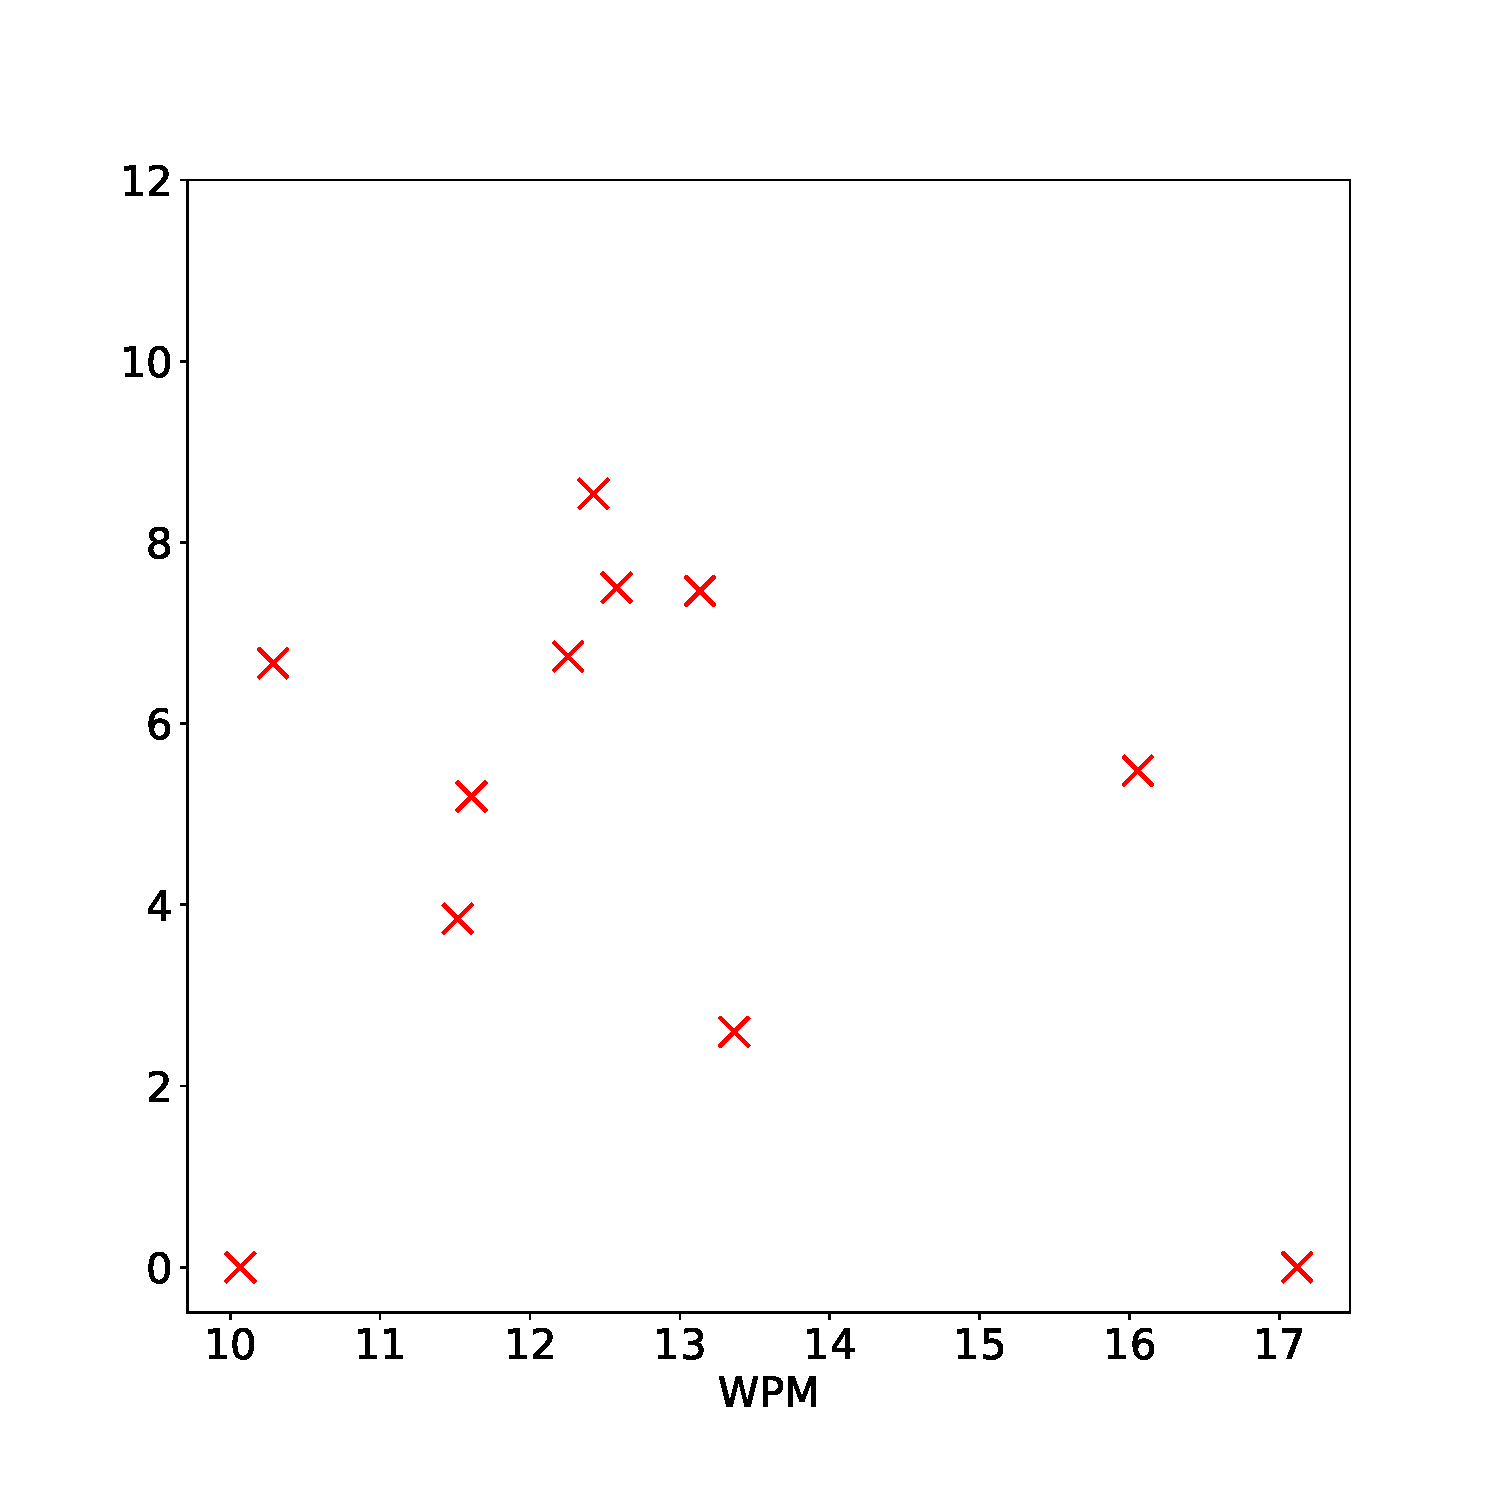
\includegraphics[width=0.6\textwidth]{user_error3_4.pdf}}
    }
    \caption{(a) shows the percentage of characters calculated with the MSD from wrong words that were not immediately corrected with the word suggestions. (b) is the same as (a) but errors from ``the'', ``in'' and ``more'' are ignored. (c) is the same as (a) but not with characters, but with the words as whole. (d) is the same as (b) but not with characters, but with the words as a whole}
    \label{fig:error_user}
\end{figure}
\fi
\begin{figure}[H]
    \centering
    \makebox[\textwidth][c]{
        \centering
        \subbottom[Not immediately corrected words' characters\label{fig:error_user:error_user1}]{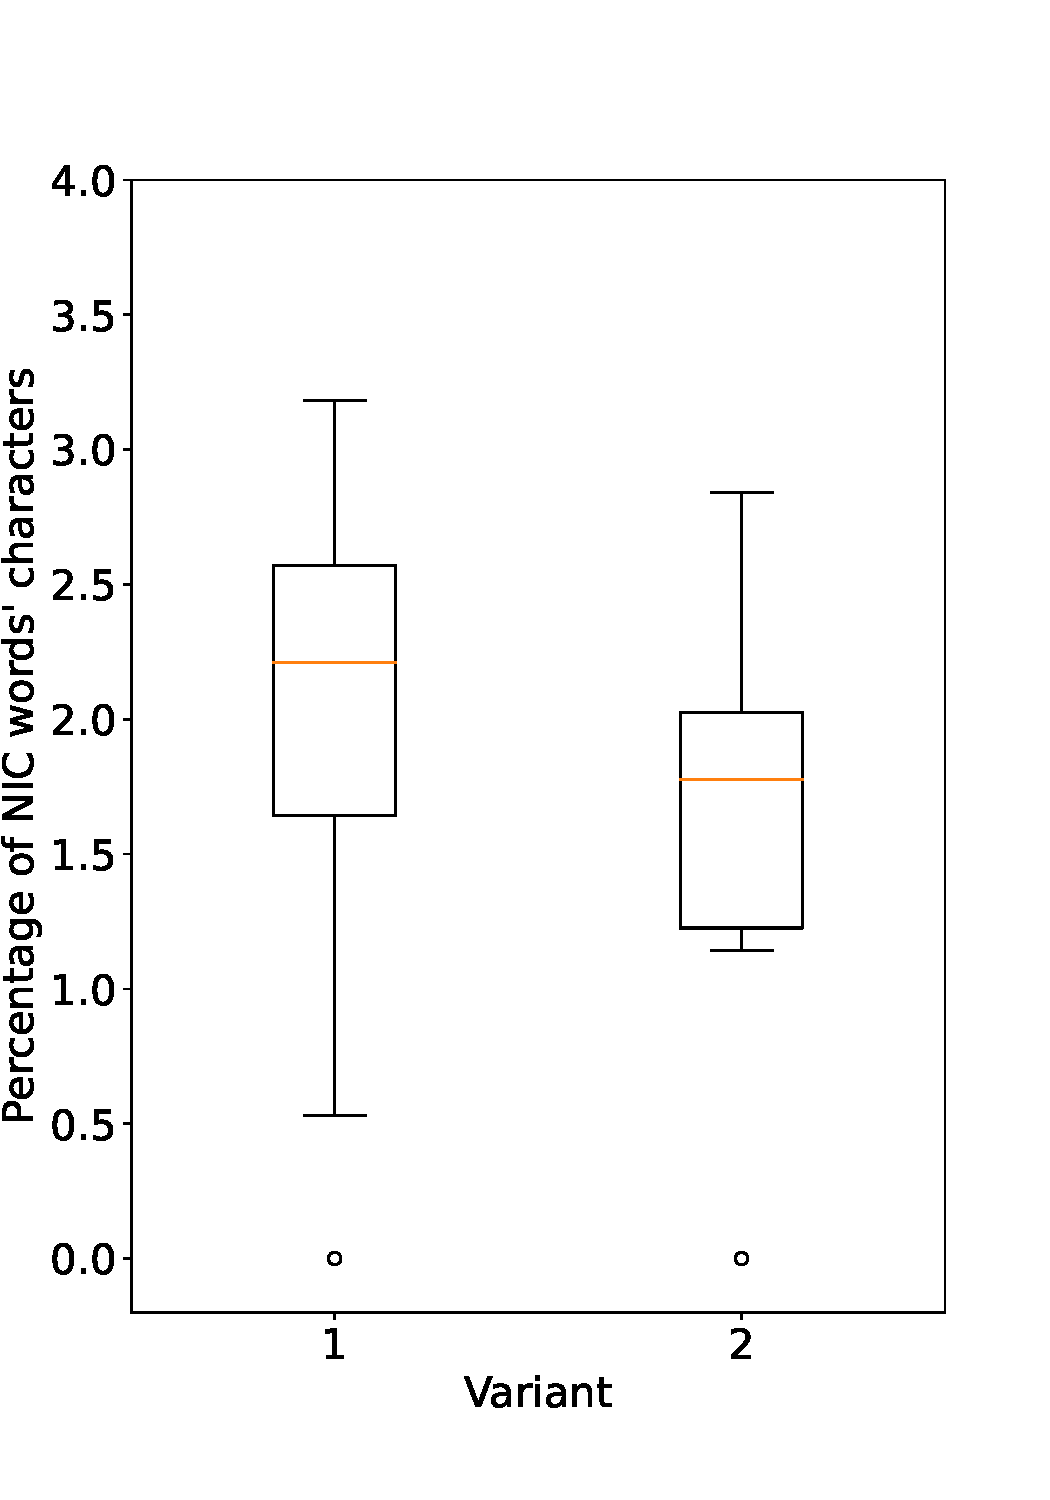
\includegraphics[width=0.45\textwidth]{user_error3_12.pdf}}
        \subbottom[Not immediately corrected words\label{fig:error_user:error_user2}]{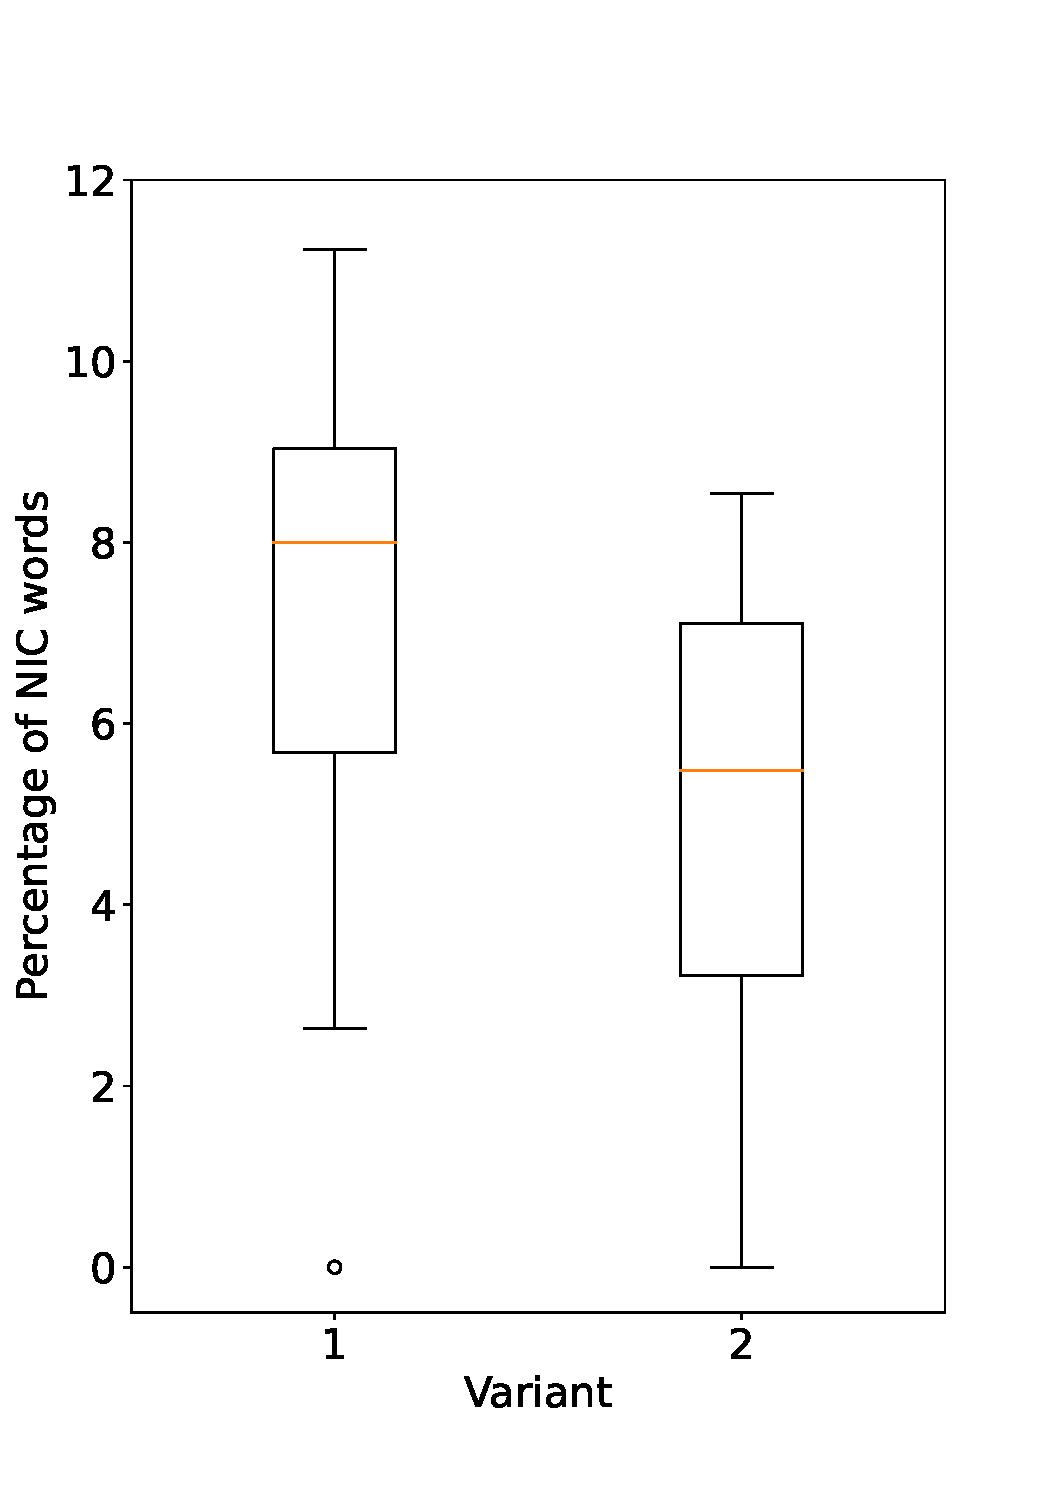
\includegraphics[width=0.45\textwidth]{user_error3_34.pdf}}
    }
    \caption{(a) shows the ratio of NIC words' characters to all inputted characters. (b) shows the ratio of NIC words to all inputted words. The left boxplots in (a) and (b) are with all NIC words, the right ones are without considering ``the'', ``in'' and ``more''.}
    \label{fig:error_user}
\end{figure}

%In \cref{fig:error_user:error_user1} and \cref{fig:error_user:error_user2} we calculate the MSD of the words, a participant did not correct, although they had the chance to do it with the keyboard's suggestions. On the y-axis, we look at the percentage, that these characters make up in comparison to all characters the participant had to write in all 15 phrases. In \cref{fig:error_user:error_user1} we look at all wrong words. But a lot of the errors came from the words ``the'', ``in'' and ``more'', that could have been prevented as mentioned before. Therefore, in \cref{fig:error_user:error_user2} we look at the errors without considering these three words.\\
In \cref{fig:error_user:error_user1} we can see that the percentage of NIC words' characters lies between about 0-3.5\%. We can observe that the percentage decreases a bit from the left to the right box. In \cref{fig:error_user:error_user2} the percentage is between about 0-11.5\%. It also drops if we do not consider the three mentioned words. Overall, the percentages are much higher when working with words instead of the characters. This is because we use MSD. If a word is wrong, most of the time, our keyboard will not write a totally wrong word, if the gesture is right to some extent. It will consist of similar letters as the right word. Therefore, not the whole word's characters will be counted into the MSD.\\
%One thing that can be observed is, that in the two lower figures of \Cref{fig:error_user} the percentage values are almost the same as in the two upper ones. This means that the words that were not corrected, have on average about the same length as the average length of all words from the respective 15 phrases is.\\
%One thing that can be observed at the left figures of Fig \Cref{fig:error_user} is that apart from one exception the percentage rate of not corrected words/characters is higher at lower WPM than it is at higher WPM. One obvious reason for this could be, that if words early in phrases were not corrected, a user had to delete the whole phrase back to the wrong word, and had to write all again. Therefore, it would make sense, that the faster participants made fewer errors, hence their risk of not correcting a word in the beginning of a phrase is lower. And then, they would not decrease their average WPM so much.

To take another look at the participants' attention, we want to calculate the value of participant conscientiousness. As for the total ER, we also take the formula for the participant conscientiousness value from the paper of Soukoreff and MacKenzie \cite{10.1145/642611.642632}:
\begin{equation}
    Participant\ Conscientiousness = \frac{IF}{INF + IF}
    \label{eq:total_er}
\end{equation}

Normally, they would take the values of $IF$ and $INF$ as mentioned in Section \ref{sec:total_er} (not as we took them but as Soukoreff and MacKenzie \cite{10.1145/642611.642632} defined them). We think for this calculation, we should not use characters but words. Thus, for $INF$ we count all the words not immediately corrected by a participant and for $IF$ the words that were corrected by using the keyboard's suggestions. We think that the calculation makes more sense this way when looking at our keyboard, which writes whole words and not single characters most of the time. It shows us, if the participants were attentive and used the keyboard's word suggestion when needed. A score of 100\% would be perfect. This would mean that a participant has corrected every word with the word suggestions, if it was possible and needed. The average value we get here is 66.28\%, which means about two third of the words that could be corrected with the suggestions, were corrected this way. The worst value is 33.33\% and the best value a participant achieved is 100\%. In our opinion, this score is not too bad. A lot of the participants are not used to word-gesture-keyboards and do not work in or use VR that much. We think if they used the keyboard over a longer period of time, they would get used to the words that are sometimes harder for the keyboard to get as best match and would pay more attention to use the word suggestions then. It is interesting that if we ignore the words ``the'', ``in'' and ``more'', the average value decreases to 63.73\%. This is an indication that the participants have already gotten used to correct these words by using the word suggestions.

\subsubsection{Word Not Found Error Rate}
Here, we do not want to see if a participant was paying attention or not but rather if our algorithm finds the right words most of the time. We count all the words that were neither the best match nor in the word suggestions, such that a participant had no chance to get this word right the first time. If this happened multiple times to a word, we count it in every time. We decide to name this error rate the word not found (WNF) error rate, because our algorithm was not able to find the right word.
\iffalse
\begin{figure}[H]
    \makebox[\textwidth][c]{
        \centering
        \subbottom[with characters\label{fig:error_system:error_system1}]{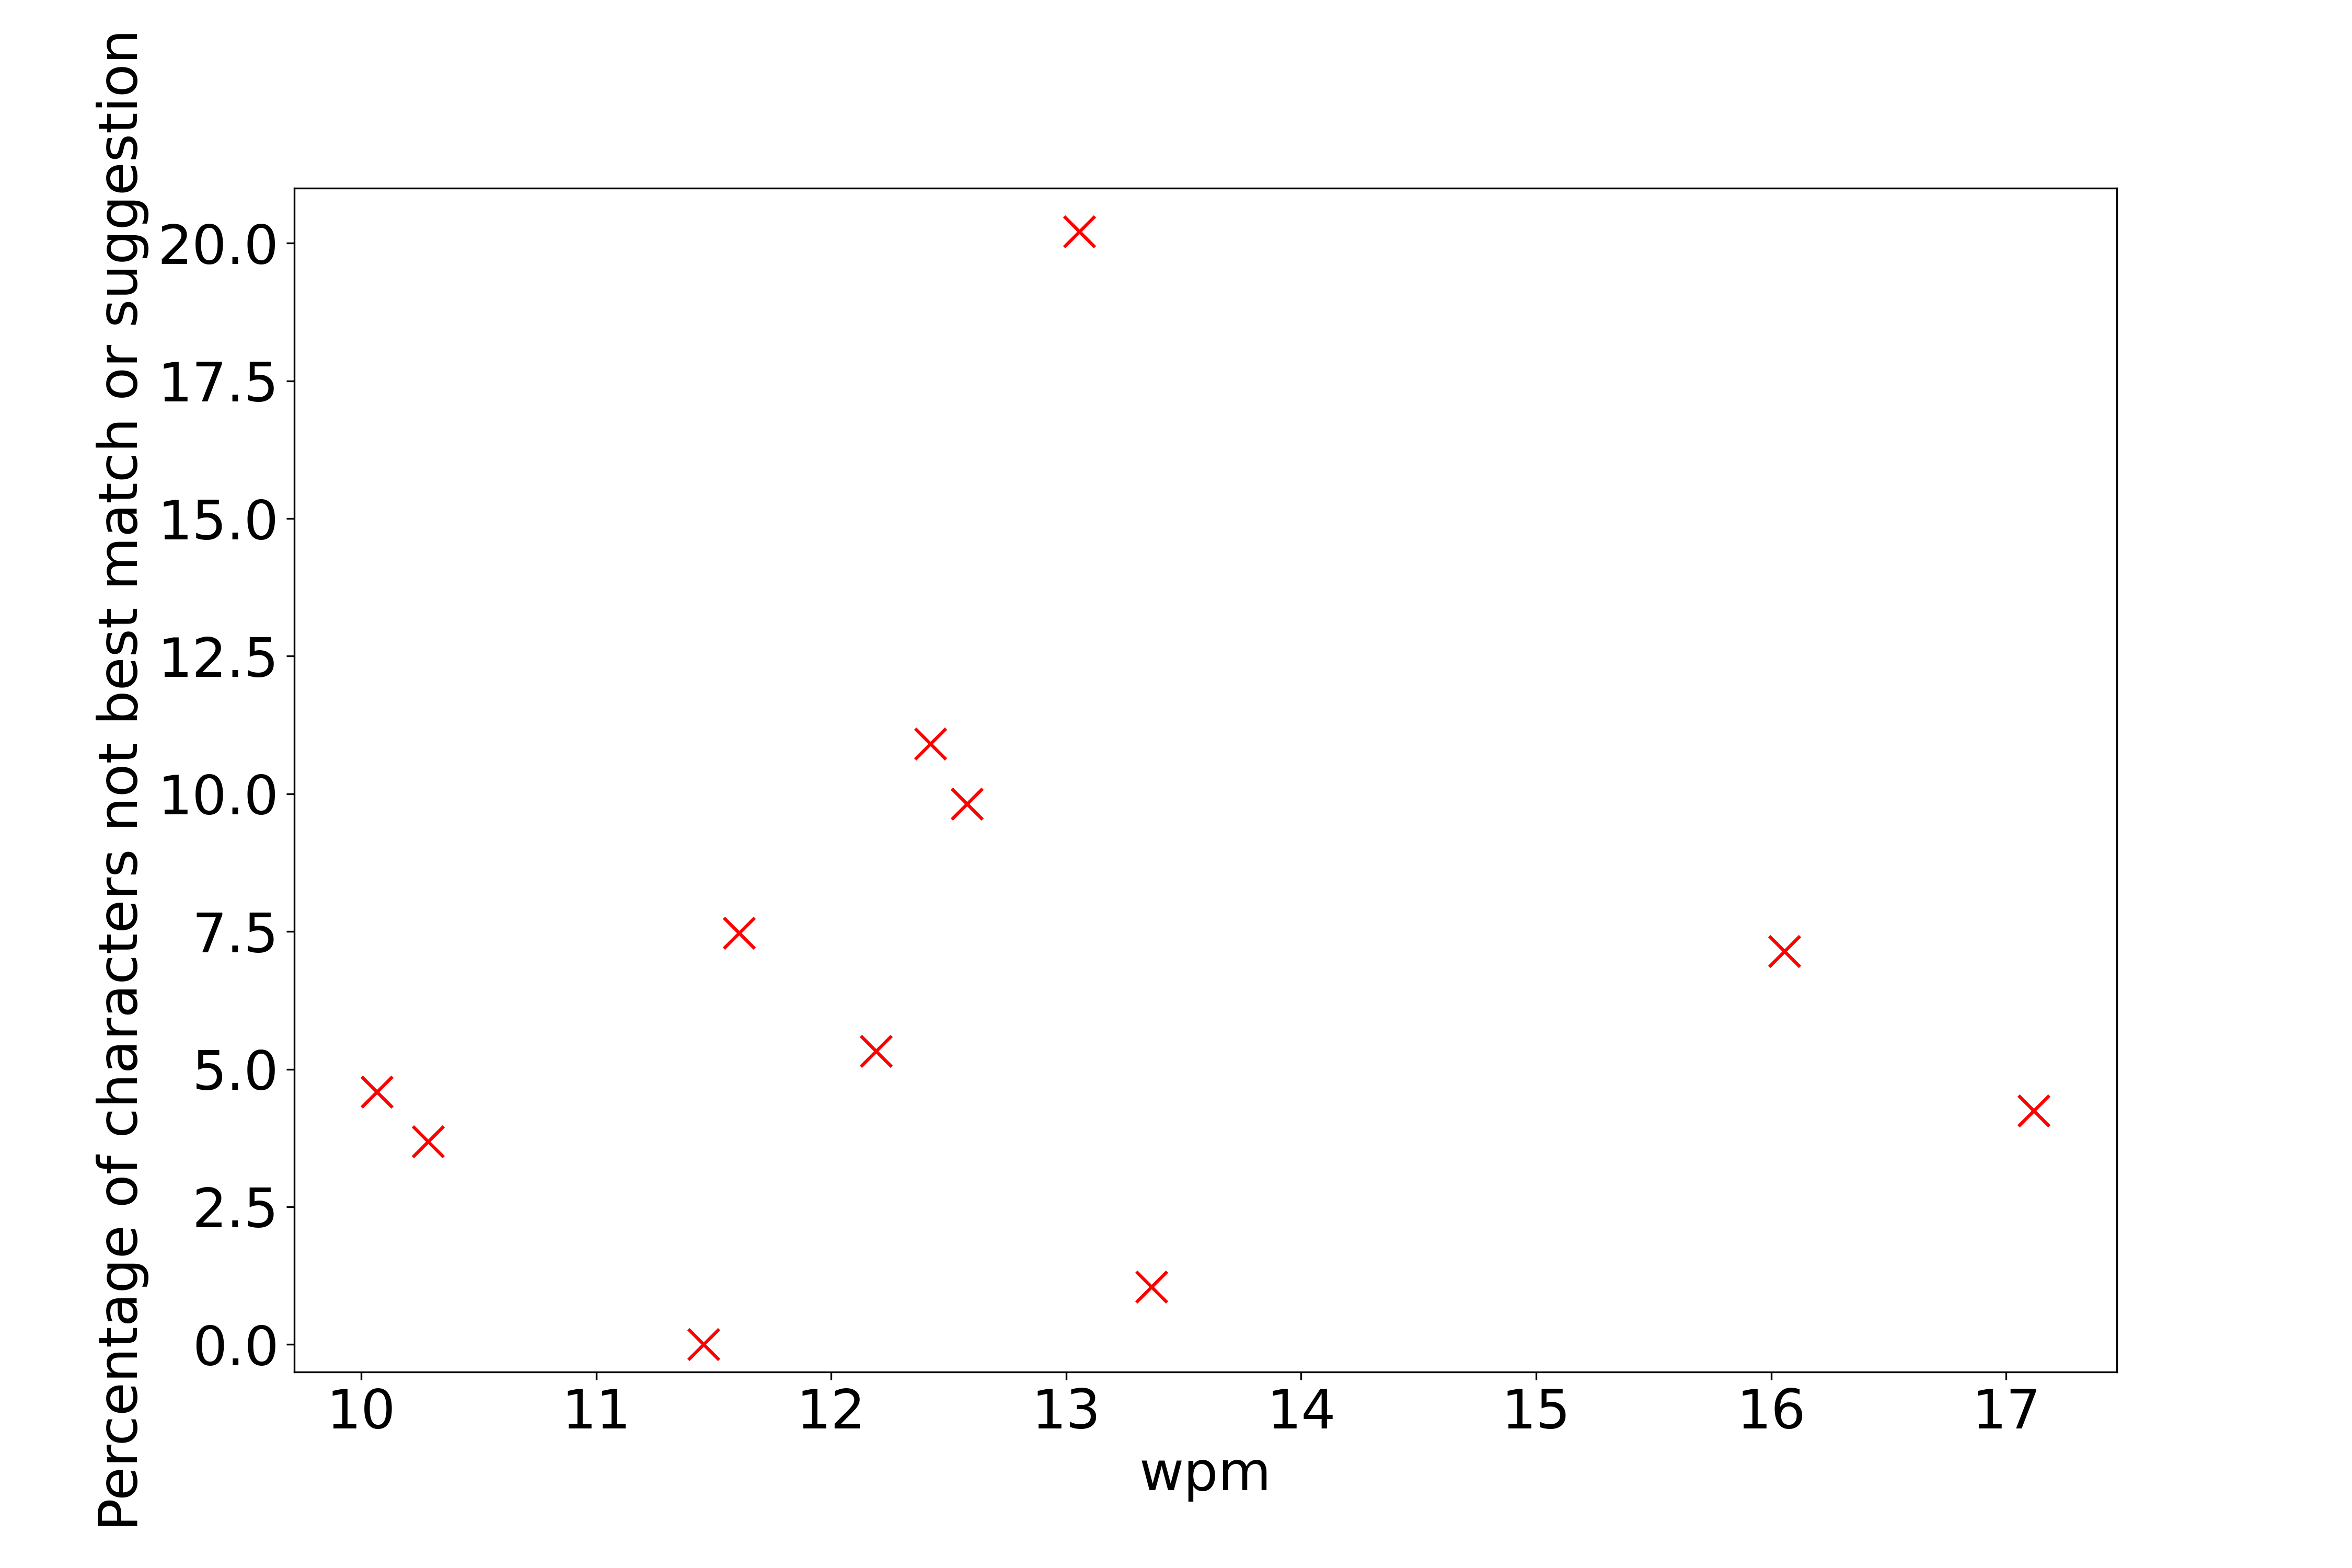
\includegraphics[width=0.6\textwidth]{system_error2_1.png}}\hspace{-3.0em}
        \subbottom[with words\label{fig:error_system:error_system2}]{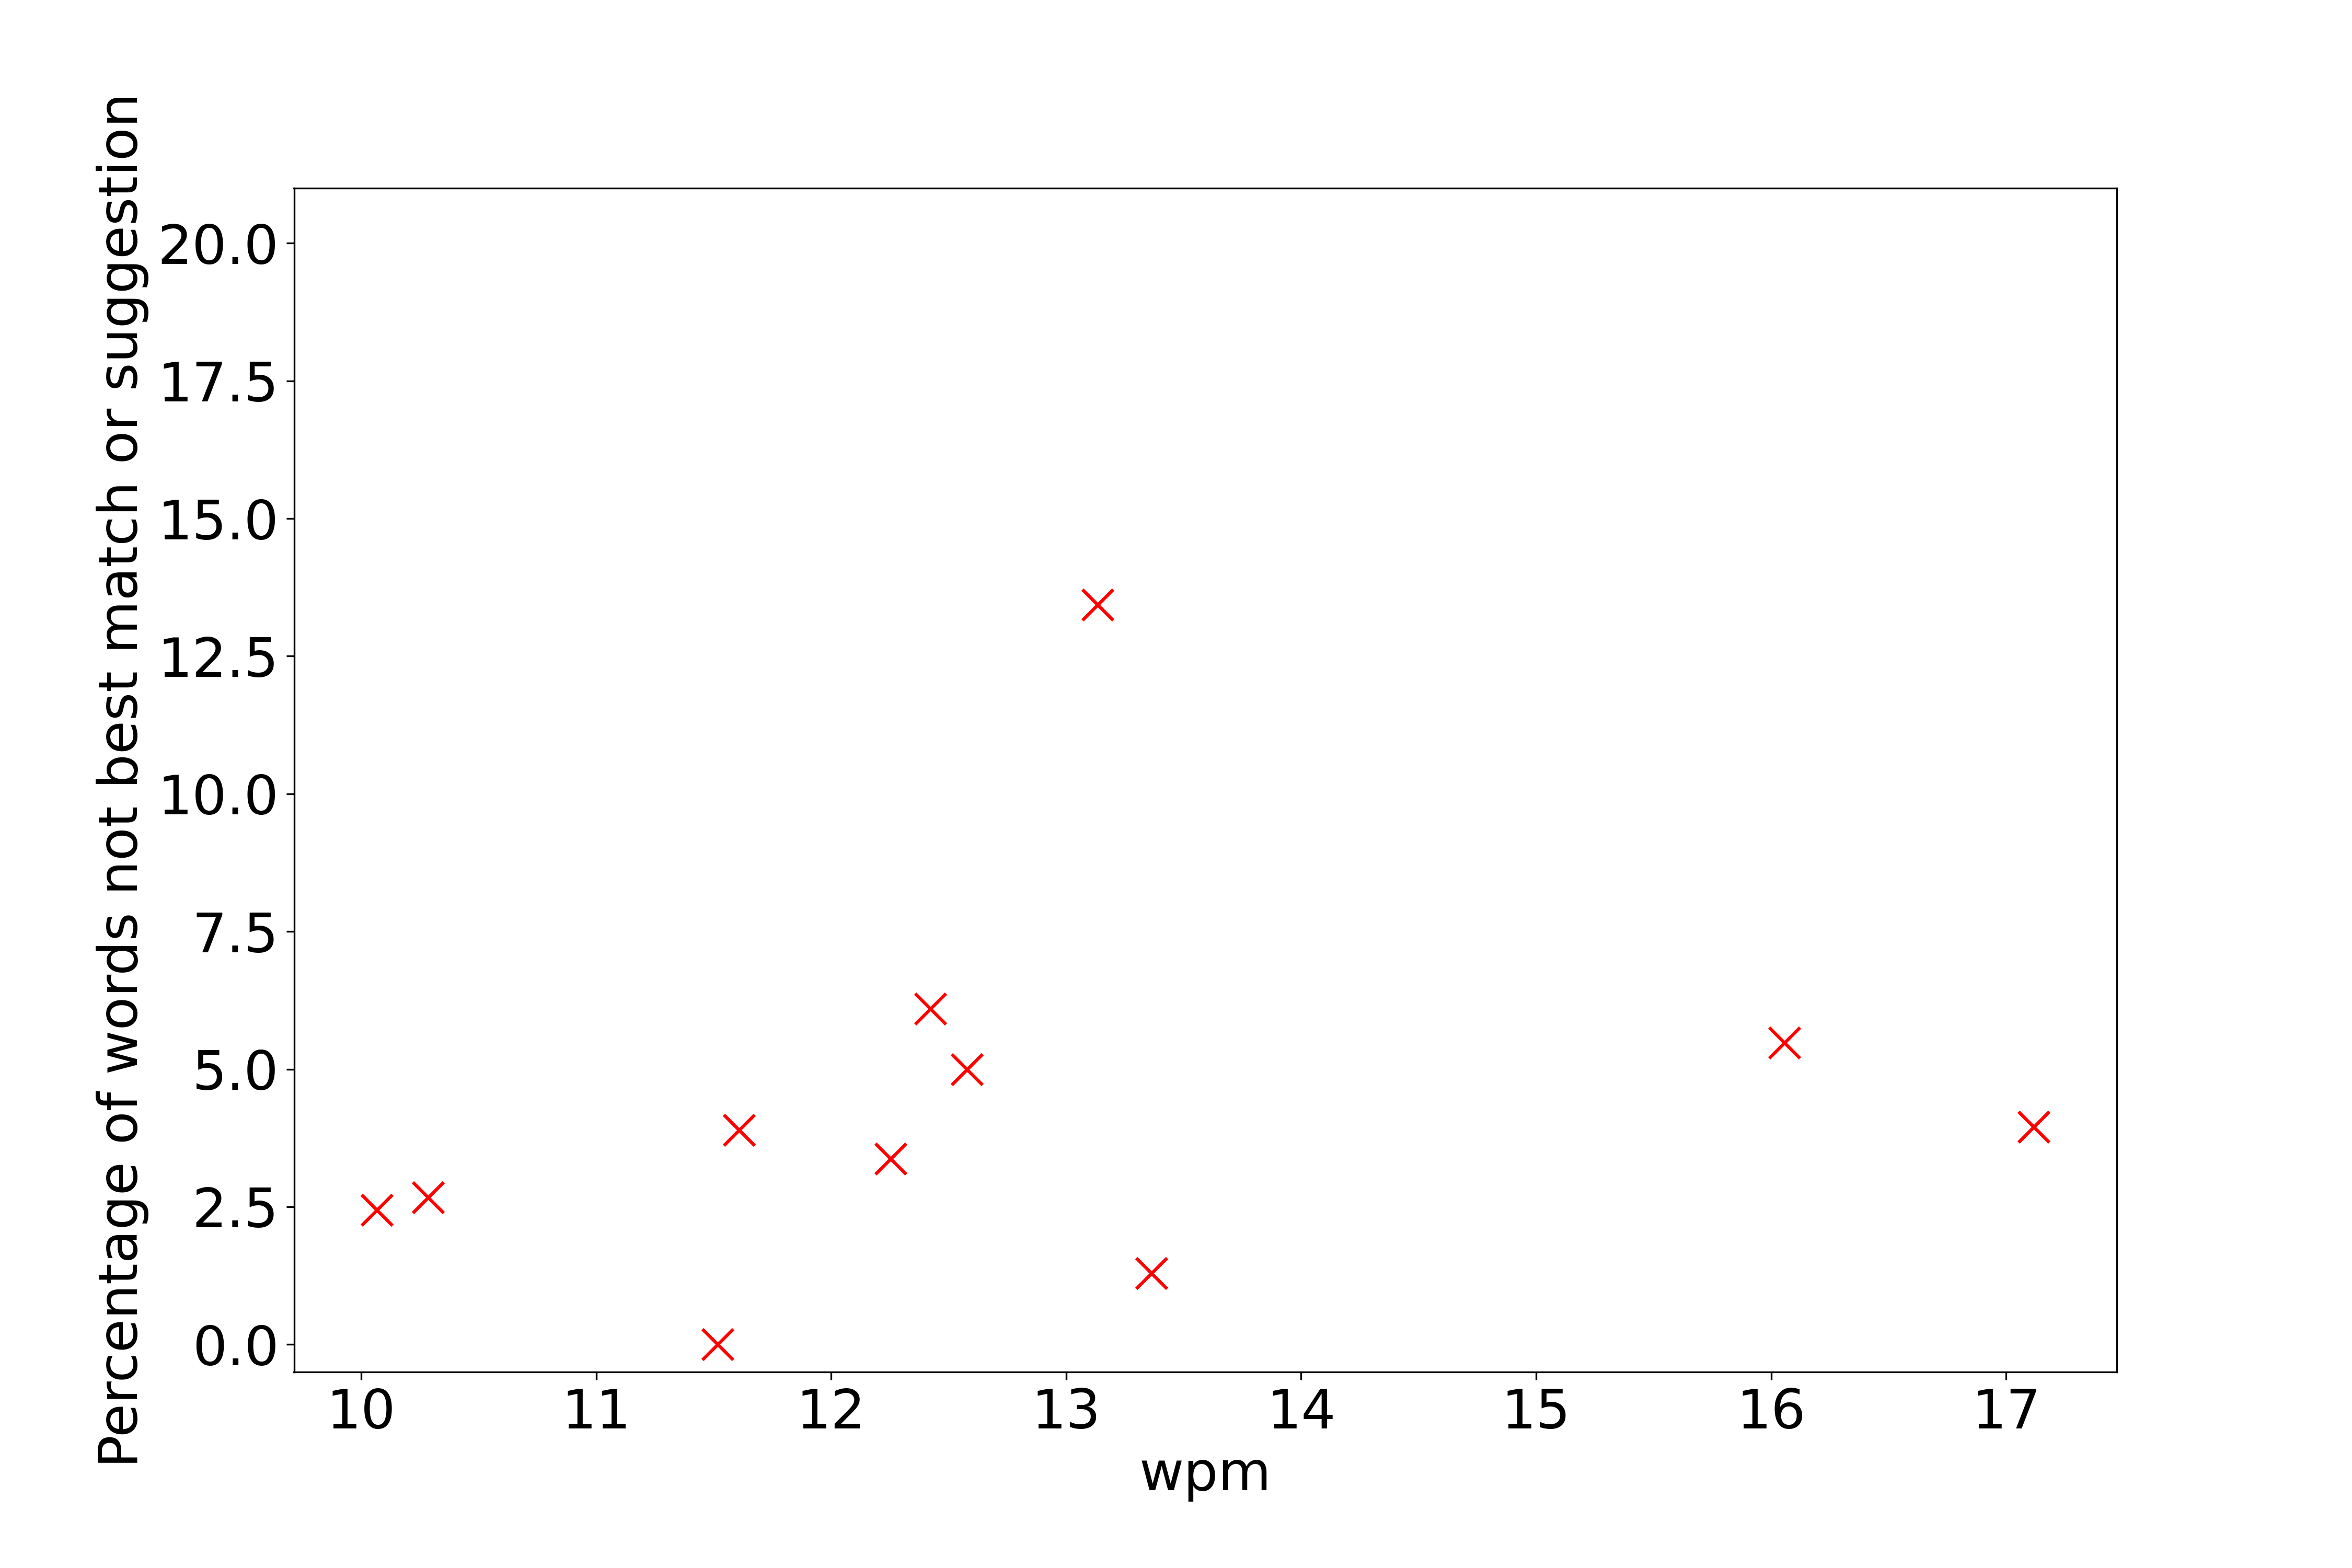
\includegraphics[width=0.6\textwidth]{system_error2_2.png}}
    }
    \caption{percentage of characters/words that were not found by the system neither as best match nor as suggestion}
    \label{fig:error_system}
\end{figure}
\begin{figure}[H]
    \centering
    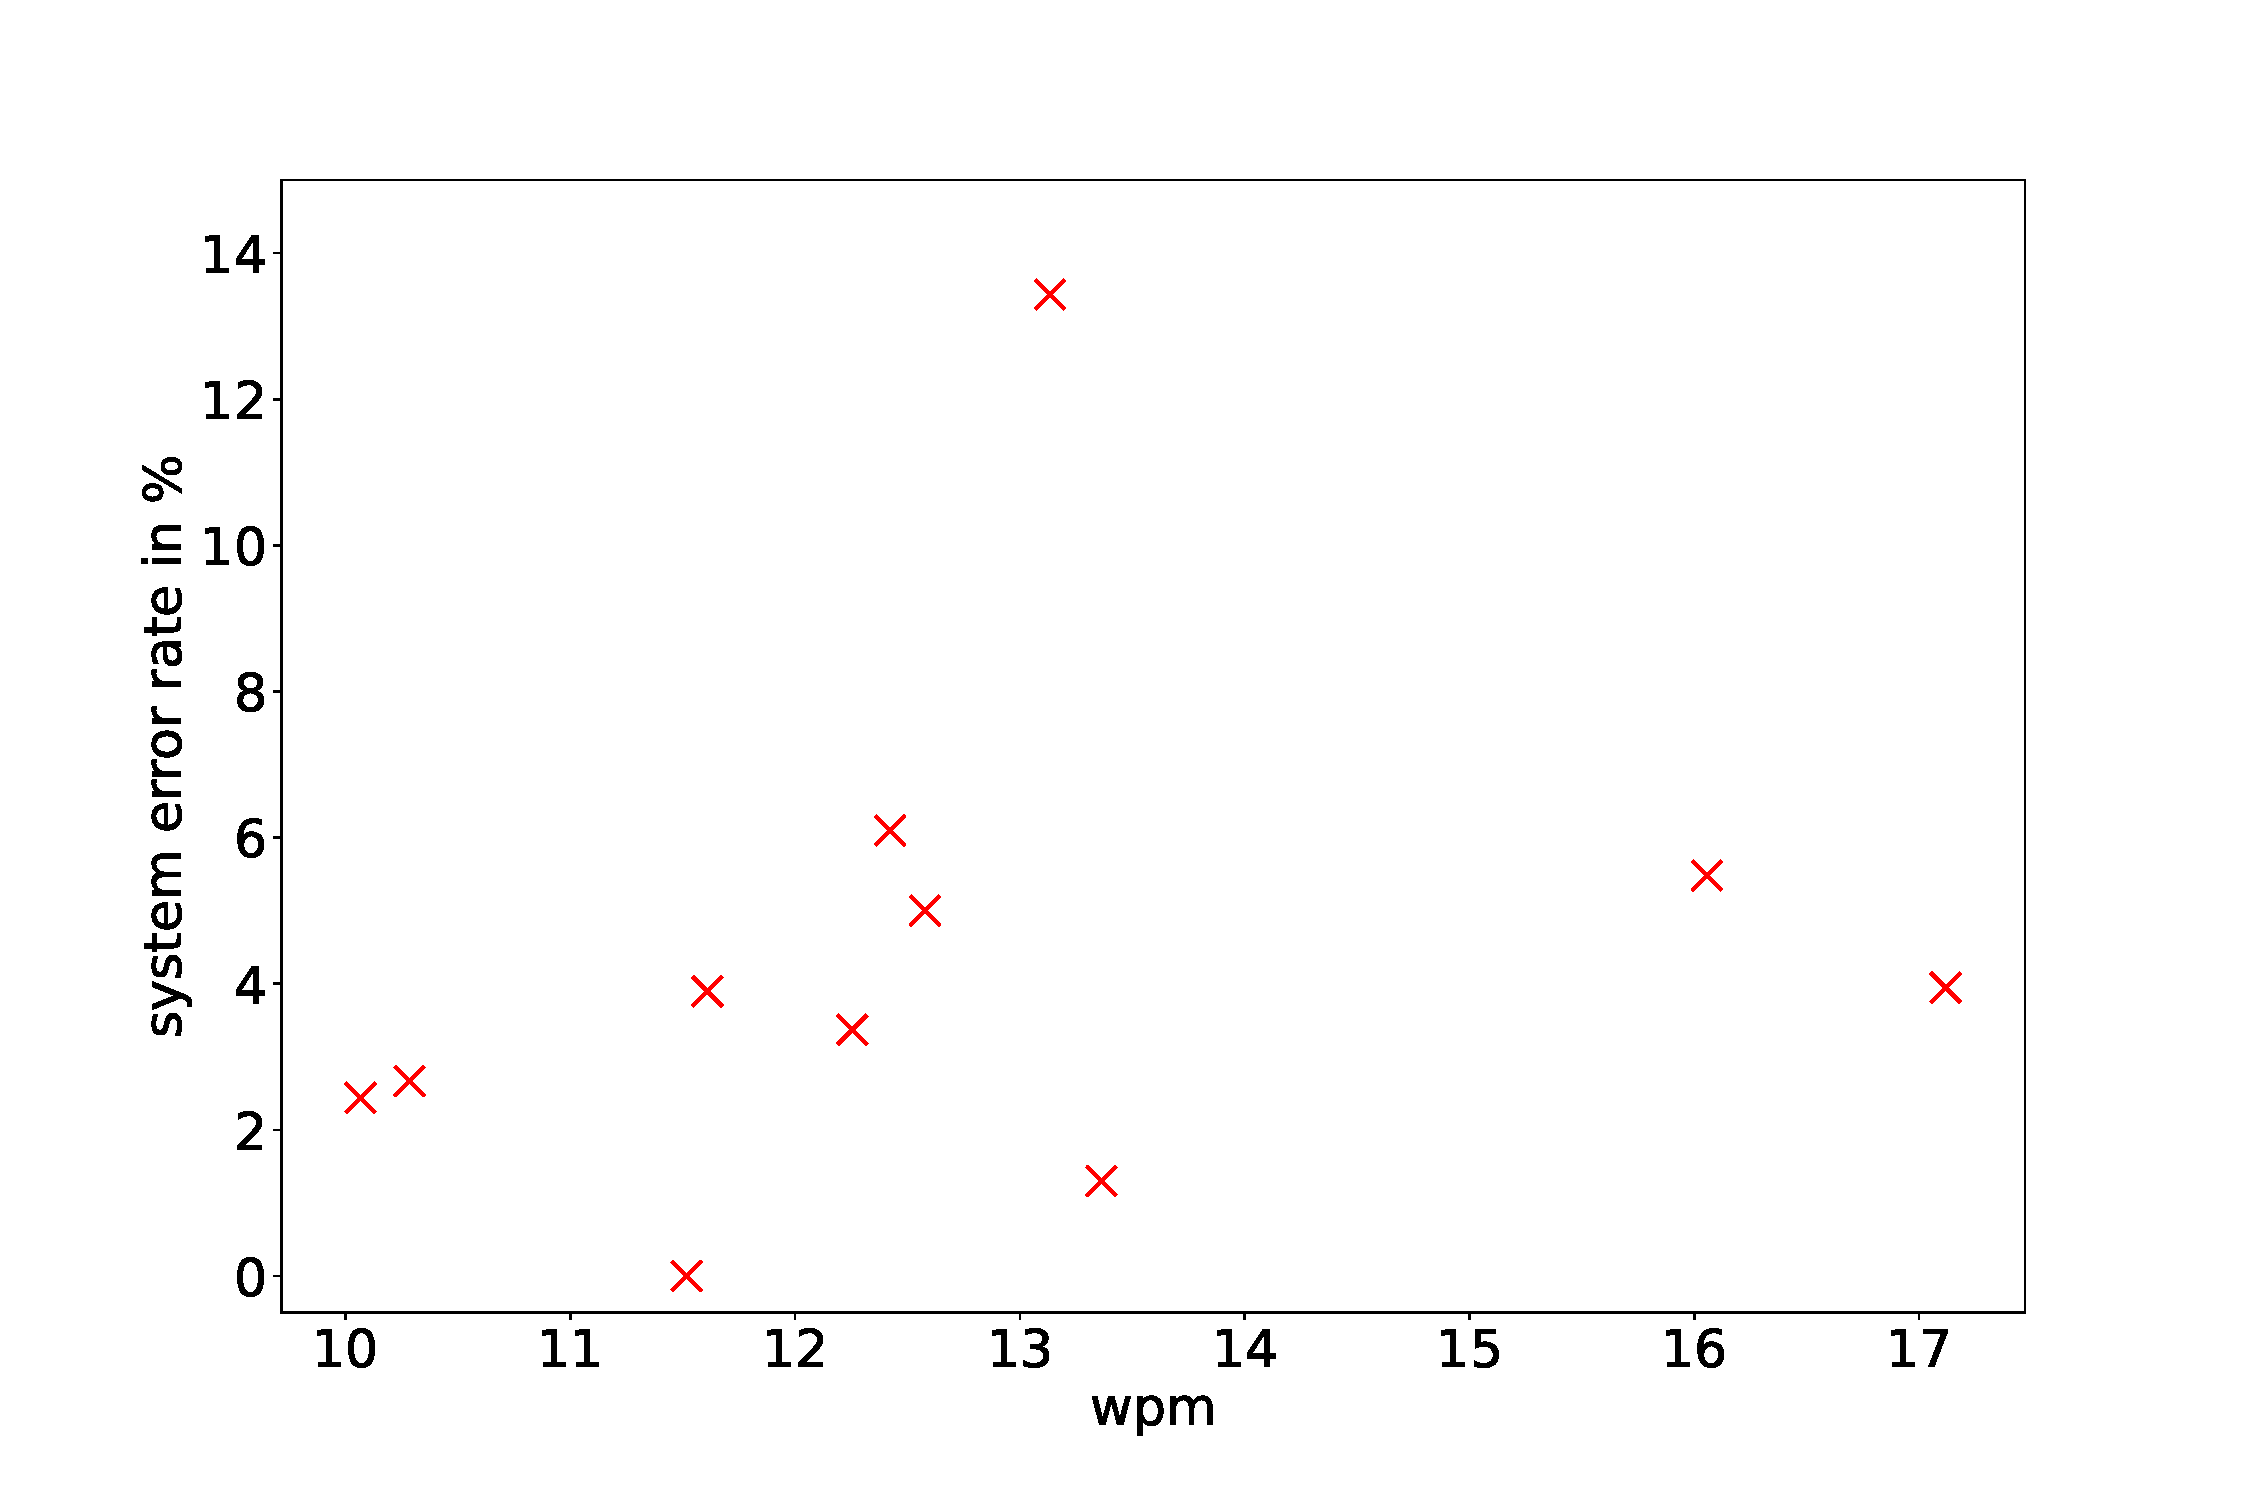
\includegraphics[width=0.8\textwidth]{system_error2_2.pdf}
    \caption{percentage of words that were not found by the system neither as best match nor as suggestion}
    \label{fig:error_system}
\end{figure}
\fi
\begin{table}[H]
    \centering
    \caption{Word not found error rate for each participant and the overall average}
    \begin{tabular}{cc} \toprule
        participant&total ER\\ \midrule
        1&0.00\%\\
        2&3.37\%\\
        3&13.43\%\\
        4&3.90\%\\
        5&5.00\%\\
        6&2.67\%\\
        7&6.10\%\\
        8&5.48\%\\
        9&1.30\%\\
        10&3.95\%\\
        11&2.44\%\\\bottomrule
        average&4.33\%\\
        \bottomrule
    \end{tabular}
    \label{tab:wnf_er}
\end{table}
In \Cref{tab:wnf_er} we can see that the average WNF error rate is 4.33\%, which means that about every 23rd word could not be written in the first attempt. While the average length of a word of the phrases we used is 4.16, the average length of a word the system has not found in the first try is 7.03. This seems to indicate that words with a length way bigger than the average one are more error-prone. We think this makes sense because the longer the word, most of the time, the larger the gesture. Deviations from the perfect graph are harder to prevent if one draws a large gesture instead of a small one and then the system might not output the right word.
%We can see, that in \cref{fig:error_system:error_system1} the percentages are much higher than in \cref{fig:error_system:error_system2}. This means that the words, which the system did not find a word, need to be longer than an average word in the written phrases. A reason for this might be, that often gestures for long words did not succeed. If a participant made some little curves too much in a gesture for a long word, the chances are lower, that the system can detect the right word, whereas for a small word the chance is higher, that the word gets found. Because the gesture can be much shorter and therefore fewer inaccuracies from a participant will happen.\\
%For the WPM and the percentages we can not detect any correlation. It seems, that these two values are not connected with each other. 

\subsection{Feedback}
The full list including all verbatim feedback from every participant can be found in the appendix. Here, we just want to highlight the most frequently addressed points.\\
Some participants find the best matches and suggestions sometimes confusing. The most mentioned example is that ``thee'' is preferred over ``the''. The visualization of spaces or the current position are another thing that is frequently addressed. Some participants find it unclear where the cursor is, hence if a space is missing or not. They suggest to implement some kind of visual indication that indicates where the cursor currently is. We can say that this problem existed in the evaluation environment but vitrivr-VR, the program that our keyboard is manly developed for, has these kinds of cursor visualizations. We also got a lot of praise and most of the time we saw a cheerful face when the VR headset got taken off. Some find it surprisingly intuitive and others have a good feeling about using it.

\subsection{Improvements}
Because of the feedback and some observations, we decide to do one more implementation. It is not a big change in the code, but can still be fairly useful. We have the problem, that for example, ``thee'' is prioritized before ``the'', which does not make much sense, because ``the'' is used far more in plain language. Because the word list we are currently using is ordered by the frequency of the words, we let this influence the best match and word suggestions. Now, if two or more words have the same highest score, the one that is highest in the word list will be taken, followed by the second highest and so on, until a word with a lower score comes next. This will prevent the problem with some words listed in Table \ref{tab:error_words}.